\documentclass[12pt,a4paper]{article}
\usepackage[utf8]{inputenc}
\usepackage[T1]{fontenc}
\usepackage{amsmath,amssymb}
\usepackage{graphicx}
\usepackage{booktabs}
\usepackage{longtable}
\usepackage[margin=2cm]{geometry}
\usepackage{setspace}
\usepackage{caption}
\usepackage{subcaption}
\usepackage{hyperref}
\usepackage{textcomp}
\usepackage{siunitx}
\usepackage{float}
\usepackage{xcolor}

\onehalfspacing

\title{\textbf{Automated analysis of nuclear emulsion exposed to
\textsuperscript{124}Xe\textsuperscript{+54} at about 300\,MeV per
nucleon at the JINR Nuclotron}}

\begin{document}
\begin{titlepage}
\begin{center}

\includegraphics[width=4cm]{jinr_logo.png}\\[0.5cm]
{\Large \textbf{JOINT INSTITUTE FOR NUCLEAR RESEARCH}}\\[0.3cm]
{\large Veksler and Baldin Laboratory of High Energy Physics}\\[0.5cm]
{\color{blue}\hrulefill}\\[0.5cm]
{\Huge \textbf{FINAL REPORT}}\\[0.3cm]
{\Large On the START Program}\\[1cm]
{\Huge \textbf{Automated analysis of nuclear emulsion exposed to
ions \textsuperscript{124}Xe\textsuperscript{+54} at about 300\,MeV per
nucleon at the JINR Nuclotron}}\\[1cm]
\textbf{Student} \\[1mm]
Ronald Lawrence Jeyaseker \\
The American College \\
Madurai \\
India
\end{center}

\vspace{0.5cm}
\begin{center}
\textbf{Supervisors} \\[2mm]
Dr. Pavel Igorevich Zarubin \\
Dr. Andrei Aleksandrovich Zaitsev \\
Dr. Marimuthu Natarajan \\[1cm]
\textbf{Participation period:} \\
May 4 -- June 27, 2026
\end{center}

\vfill
\begin{center}
Dubna, 2026
\end{center}
\end{titlepage}

\begin{abstract}
The article presents results of an analysis of a nuclear emulsion
exposed in March 2026 with an extracted beam of
\textsuperscript{124}Xe\textsuperscript{+54} ions at around 300\,MeV per
nucleon at the JINR Nuclotron. The primary objective was to determine
the beam profile and its uniformity, and to locate the Bragg peak
position for applied research in electronic components and radiation
biology. Three stacks of 8--10 emulsion layers of 60\,\si{\micro\meter}
thickness each poured onto a 2\,mm thick glass base measuring
$9\times12$\,cm\textsuperscript{2}, were exposed transversely to the
beam, allowing capture of the bulk of the beam and tracking of ion
deceleration until complete stop or the formation of long-range
fragments. Digital photography of approximately 80\% of each layer area
was performed using an intelligent microscope Olympus BX63, and the
frames were combined into a complete layer image using the microscope's
software. The high ionization of the ions made it sufficient to use a
4$\times$ objective lens to detect cross-sectional images of their
tracks. Counting and determination of the track parameters were
performed using ImageJ. A Gaussian Mixture Model on grain areas
resolves three particle classes corresponding to light fragments,
mid-mass fragments, and heavy residues including the primary beam.
The Bragg peak is observed at 8--10\,mm (Stack\,01) and 10--12\,mm (Stacks\,02/03) depth.
\end{abstract}

\newpage
\tableofcontents
\newpage

%===================================================================
\section{Accelerator, research goals and objectives}
\label{sec:goals}
%===================================================================

A long-term perspective at VBLHEP has been opened up with the NICA
(Nuclotron-based Ion Collider Facility) megaproject, whose primary
scientific goal is the study of quark--gluon degrees of freedom in
nuclear matter at maximum baryonic density. NICA provides extracted
and colliding beams of heavy relativistic nuclei and polarized protons
and deuterons at energies up to 4.5GeV/nucleon for extracted beams
and up to 11\,GeV/nucleon in the collider mode.

\begin{figure}[H]
\centering
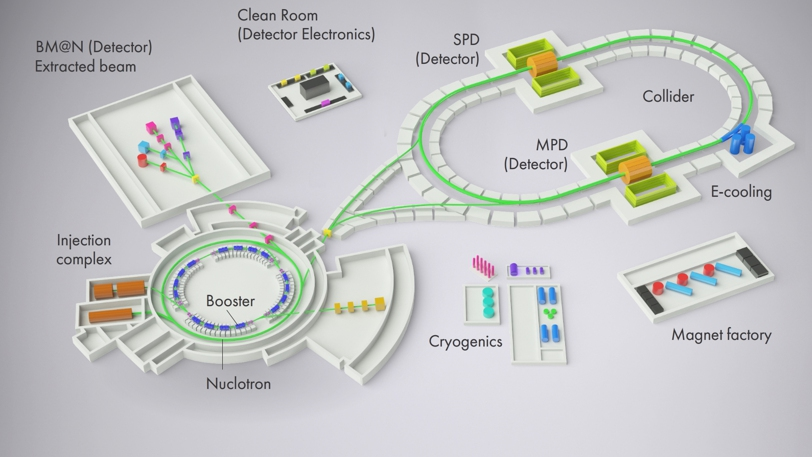
\includegraphics[width=\textwidth]{nica_scheme.jpg}
\caption{Schematic overview of the NICA accelerator complex, showing
the injection chain (ESIS/KRION, HILAC), the Booster and Nuclotron
synchrotrons, the collider rings, and the MPD and SPD detectors.
Image source: \texttt{nica.jinr.ru}.}
\label{fig:nica_scheme}
\end{figure}

\subsection{Accelerator cascade}

The NICA accelerator complex consists of several stages:

\begin{enumerate}
  \item \textbf{Electron String Ion Source (ESIS)} and/or
        \textbf{KRION-6T}: Produce highly charged ions of the desired
        species (e.g.\ Xe\textsuperscript{+54} for this experiment).
  \item \textbf{HILAC} (Heavy Ion Linear Accelerator): A new linear
        accelerator that accelerates ions to 3.2\,MeV/nucleon for
        injection into the booster. 
  \item \textbf{Superconducting Booster Synchrotron}: Accumulates and
        accelerates ions to \\ 
        600\,MeV/nucleon before transfer to the
        Nuclotron.
    \begin{figure}[H]
    	\centering
    	\includegraphics[width=0.5\textwidth]{jinr/Booster.jpg}
    	\caption{Superconducting Booster synchrotron of the NICA accelerator complex}
    	\label{fig:booster}
    \end{figure}
    
  \item \textbf{Nuclotron}: The main superconducting synchrotron,
        capable of accelerating heavy ions up to 4.5\,GeV/nucleon.
        Beams can be slowly extracted over several seconds for \\
        fixed-target experiments or injected into the collider rings.
  \item \textbf{Collider}: Two superconducting storage rings (each
        503\,m circumference) that bring counter-rotating beams into
        collision at interaction points for experiments such as
        MPD and SPD.
\end{enumerate}

\subsection{Beam extraction and the present irradiation}

For the present experiment, \textsuperscript{124}Xe\textsuperscript{+54}
ions were accelerated by the Nuclotron to approximately
300\,MeV/nucleon and slowly extracted via the beam extraction system
to the VBLHEP experimental hall. The beam energy at the irradiation
point was approximately 280\,MeV/nucleon, as determined from the
Nuclotron magnetic field settings. At this energy the ions have a
range of approximately 10--15\,mm in the emulsion--glass stack,
allowing the majority of the beam to stop within the 8--10 plate
assembly while still producing measurable signals in the downstream
plates from long-range nuclear fragments.

The extracted beam was delivered in a series of macro-pulses
(spills), each of several hundred milliseconds duration, with
typical intensities of $10^{4}$--$10^{5}$ ions per spill at the
irradiation point. The three emulsion stacks were exposed with
different numbers of cycles (1, 5, and 10 spills for Stacks~01,~02,
and~03 respectively) to provide a range of fluences for statistical
analysis.

\subsection{Applied physics programme at NICA}

Beyond its fundamental physics goals, the NICA accelerator complex
supports an extensive applied research programme:

\begin{itemize}
  \item \textbf{Radiation hardness of electronics:} Heavy-ion beams at
        energies of hundreds of MeV/nucleon are ideal for testing
        single-event effects (SEE) in microelectronics,\\ simulating the
        space radiation environment. The xenon beam used here provides a \\
        well-characterised source of high-LET radiation.
  \item \textbf{Radiation biology:} The Bragg peak of heavy ions in
        tissue-like media is exploited for hadron therapy. Measurements
        of the range and fragmentation of \textsuperscript{124}Xe in
        emulsion provide benchmark data for treatment planning codes.
  \item \textbf{Nuclear fragmentation:} The breakup of heavy projectiles
        in the emulsion produces a spectrum of secondary fragments
        whose yields and angular distributions are relevant for both
        fundamental nuclear physics and space radiation shielding.
  \item \textbf{Detector development:} Nuclear emulsion is itself a
        candidate detector for the NICA SPD (Spin Physics Detector)
        and for future fixed-target experiments, motivating
        quantitative studies of its response to heavy ions.
\end{itemize}

The present work directly addresses the first point (beam characterisation
for electronics testing) while contributing to the second and third by
measuring the Bragg curve and identifying fragment populations.

The specific goals of this work are:

\begin{enumerate}
  \item To determine the beam profile and uniformity of the extracted
        \textsuperscript{124}Xe beam at the \\ irradiation point;
  \item To measure the range and locate the Bragg peak of
        280\,MeV/nucleon xenon ions in the emulsion--glass stack;
  \item To classify the nuclear fragmentation products by their
        ionization density using \\ unsupervised machine learning;
  \item To compare the experimental range with SRIM simulations.
\end{enumerate}

These results are essential for the calibration of nuclear emulsion as
a detector for heavy-ion fragmentation studies, and for applications in
radiation hardness testing of electronic \\ components and in
radiobiology.

%===================================================================
\section{Nuclear Track emulsion in brief}
\label{sec:emulsion}
%===================================================================

Nuclear Track emulsion is a particle detector consisting of a photographic
gelatine layer \\ embedded with silver bromide (AgBr) crystals. When a
charged particle passes through the emulsion, it ionises the medium
along its trajectory. During chemical development, the latent image
centres in the AgBr crystals along the particle's path are reduced to
metallic silver grains, forming a visible track that can be observed
under an optical microscope. The analysis presented here is part of
the BECQUEREL project at LHEP JINR~\cite{barkas, becquerel, zarubin2016}.

The principal advantage of nuclear emulsion is its sub-micrometre
spatial resolution, which makes it uniquely suited for measuring the
interaction vertices and ranges of heavy ions in the few-hundred
MeV/nucleon energy regime. Unlike electronic detectors, emulsion
integrates the exposure passively, requires no power or readout during
irradiation, and provides a permanent record of every particle
trajectory within its volume.

\subsection{Energy loss in emulsion}

The energy loss of a heavy ion in emulsion follows the
Bethe--Bloch formula~\cite{bethe1930}:

\[
-\frac{dE}{dx} = \frac{4\pi}{m_e c^2}\cdot
\frac{n_e z^2}{\beta^2}\cdot
\left(\frac{e^2}{4\pi\varepsilon_0}\right)^{\!2}
\left[\ln\frac{2m_e c^2\beta^2}{I(1-\beta^2)} - \beta^2\right],
\]

\noindent where $z$ is the projectile charge, $\beta = v/c$ its
velocity, $n_e$ the electron density of the medium, and $I$ the mean
excitation potential. The grain size in the developed emulsion is
proportional to the local energy deposition, making it possible to
distinguish particle types by their ionization density. For a
\textsuperscript{124}Xe ion at 280\,MeV/nucleon ($\beta \approx 0.63$),
the ionization is far above the minimum, producing large, easily
detectable grain clusters.

\subsection{Emulsion composition}

The emulsion layer consists of:
\begin{itemize}
  \item AgBr microcrystals ($\sim$40\% by volume, density
        \SI{6.47}{\g\per\cm\cubed});
  \item Gelatine binder ($\sim$60\% by volume, density
        \SI{1.16}{\g\per\cm\cubed});
  \item Bulk density approximately \SI{3.3}{\g\per\cm\cubed}.
\end{itemize}

After exposure, the plates are chemically developed, fixed, and washed
following standard nuclear emulsion protocols.

%===================================================================
\section{Stack description}
\label{sec:stack}
%===================================================================

Three stacks of nuclear emulsion plates were exposed to an extracted
beam of \textsuperscript{124}Xe\textsuperscript{+54} ions in March 2026
at the JINR Nuclotron.

\subsection{Plate structure}

Each plate consists of a 60\,\si{\micro\meter} layer of nuclear emulsion
poured onto a 2\,mm thick glass substrate. The plates measure
approximately $9\times12$\,cm\textsuperscript{2}. The emulsion layer is
single-sided (one sensitive layer per plate, no backing emulsion).

\begin{figure}[H]
\centering
\includegraphics[height=0.2\textheight,keepaspectratio]{jinr/Plate.jpg}
\includegraphics[height=0.2\textheight,keepaspectratio]{jinr/PlateStack.jpg}
\caption{Left: individual nuclear emulsion plate showing the
$9\times12$\,cm\textsuperscript{2} glass substrate with the sensitive
emulsion layer. Right: assembled stack of 10 plates ready for
irradiation.}
\label{fig:plates}
\end{figure}

\begin{figure}[H]
\centering
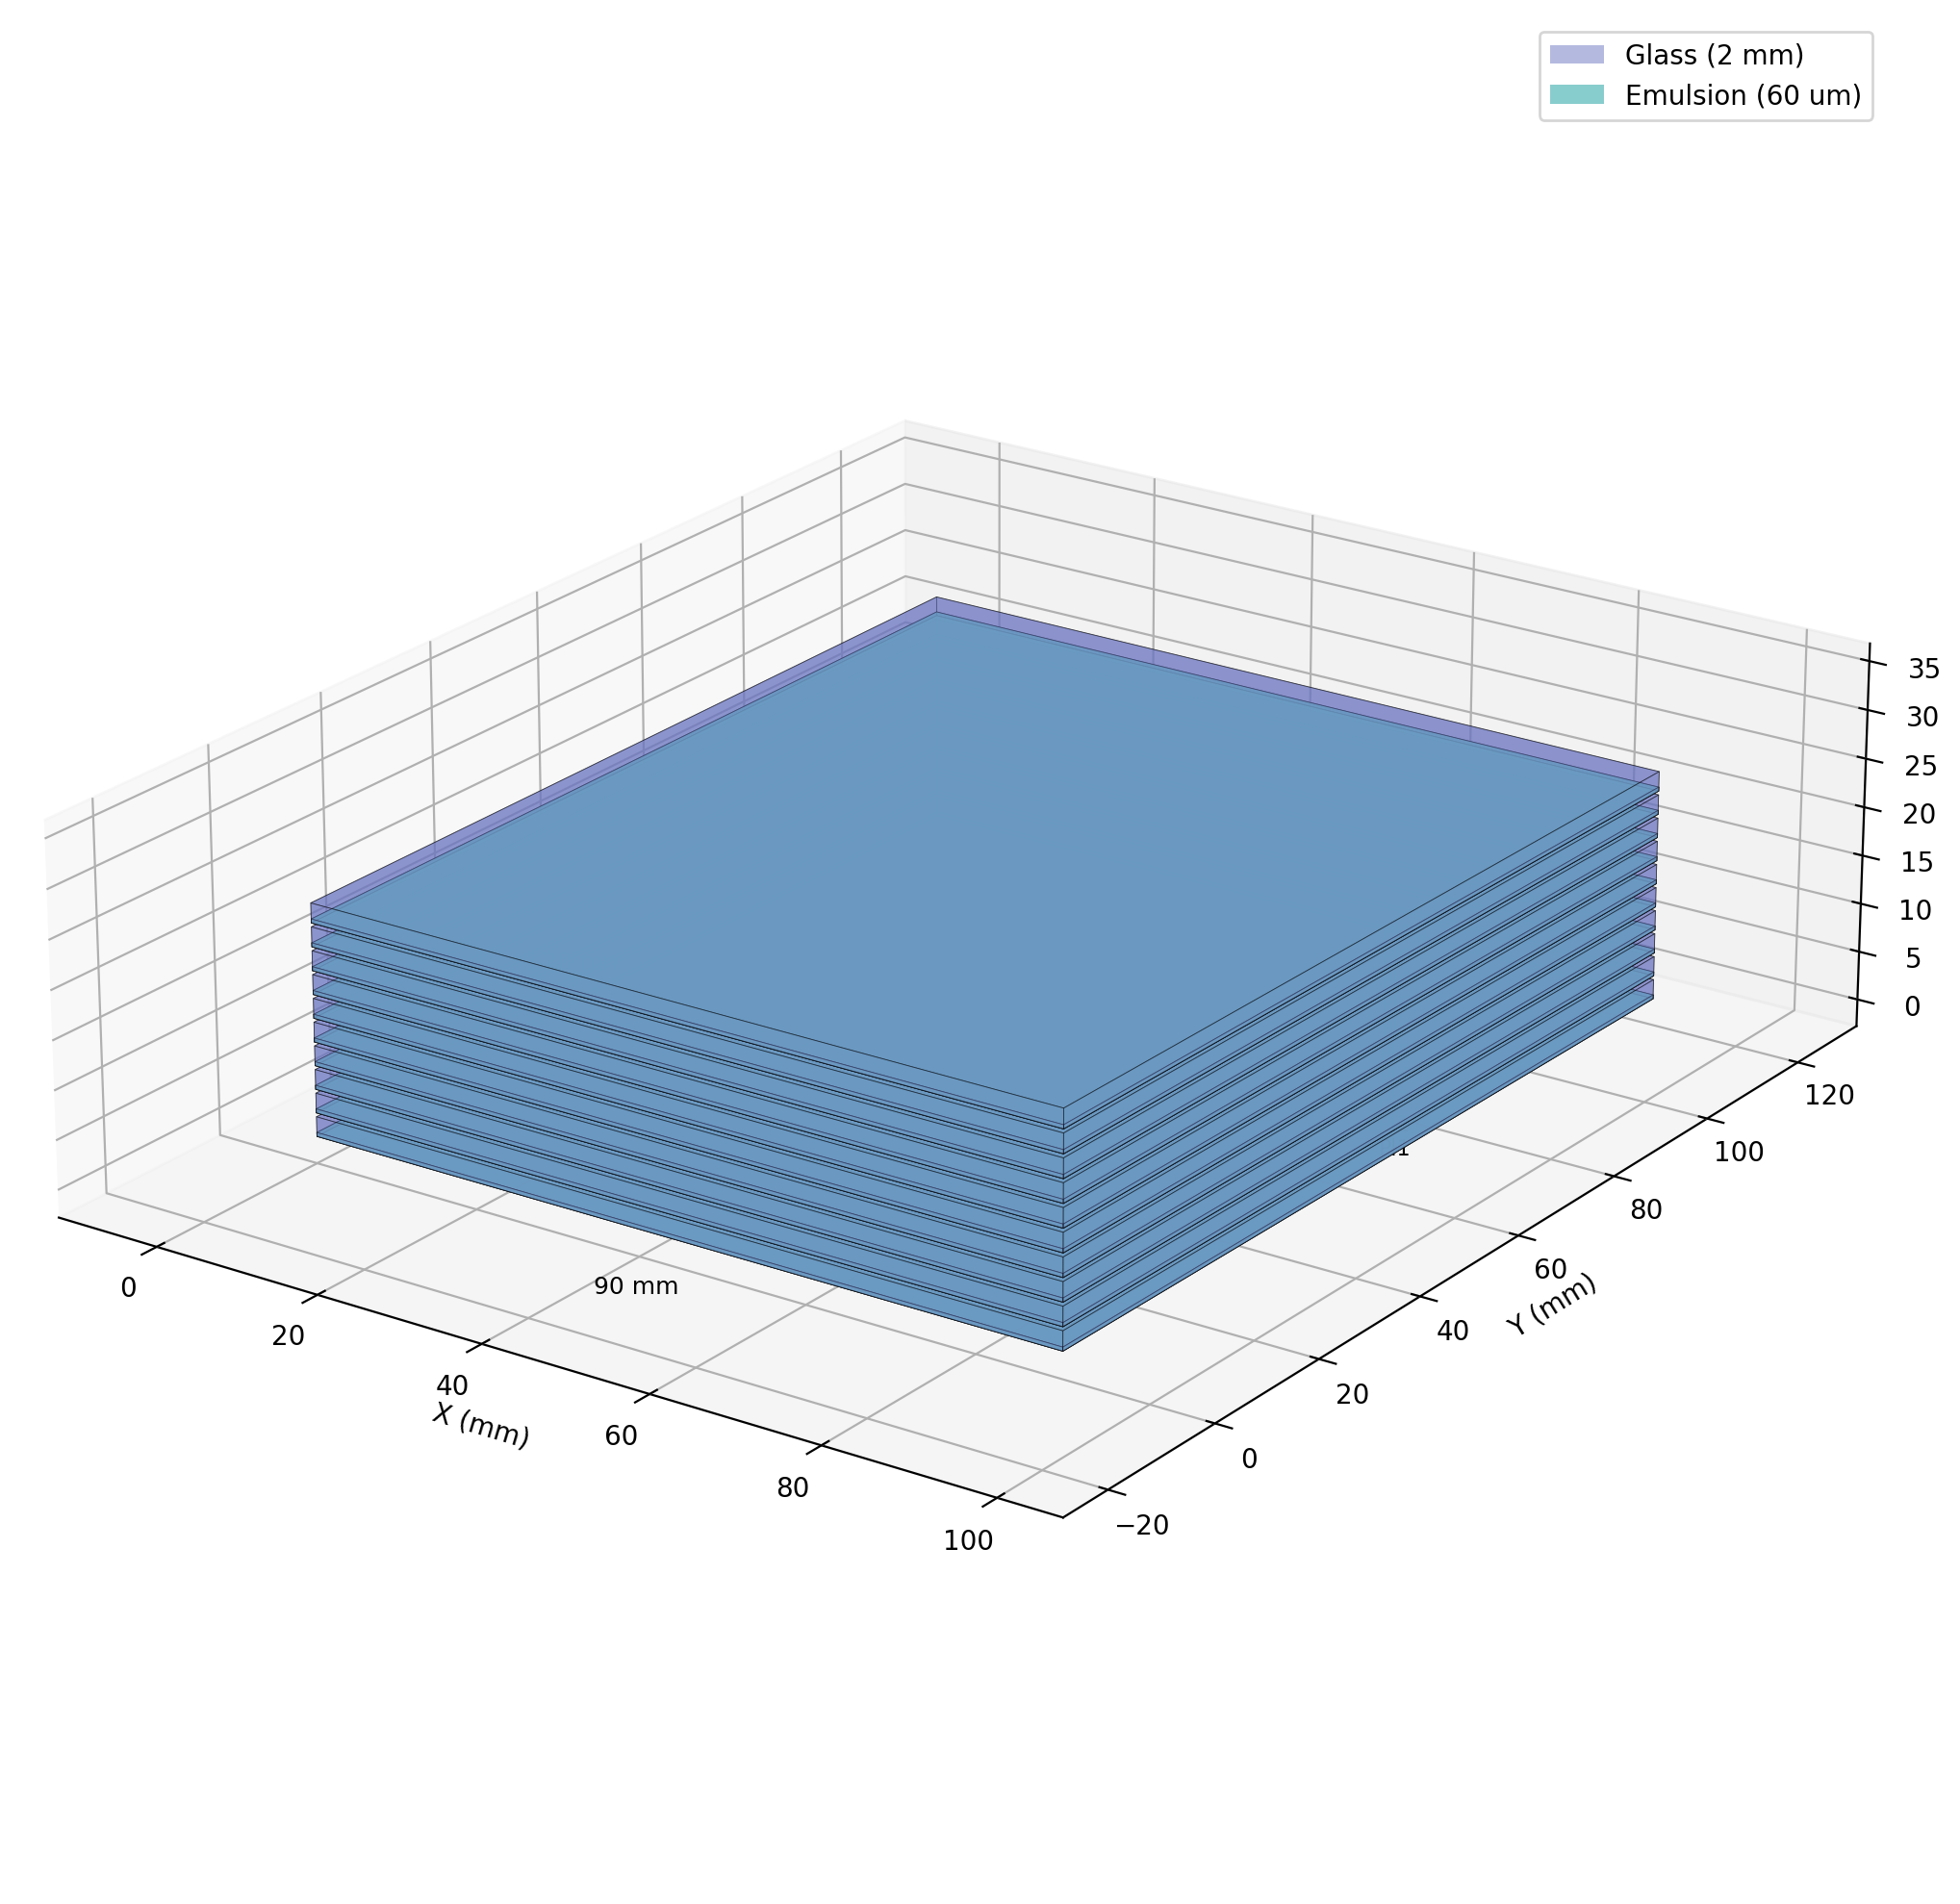
\includegraphics[width=0.65\textwidth]{./emulsion_stack_3d.png}
\caption{3D model of the emulsion stack showing 10 plates stacked
perpendicular to the beam direction (red arrow). Each plate consists
of a 60\,\si{\micro\meter} emulsion layer (teal, top surface) on a
2\,mm glass substrate (purple). The emulsion thickness is exaggerated
by $\sim$7$\times$ for visibility. Plate numbers Pl1--Pl10 are
labelled in order along the beam direction. The 9$\times$12\,cm plate
dimensions are indicated.}
\label{fig:3dstack}
\end{figure}

\subsection{Stack configurations}

\begin{table}[H]
\centering
\caption{Summary of the three irradiated stacks.}
\label{tab:stacks}
\begin{tabular}{lccccc}
\toprule
Stack & Plates & Exposure & Beam entrance & Depth range &
Scan area per plate \\
 & & cycles & plate & (mm) & (mm\textsuperscript{2}) \\
\midrule
Stack\,01 & 8 & 1 & 1\_Plate\_09 & 0.0--14.5 & $\sim$406--470 \\
Stack\,02 & 10 & 5 & 1\_Plate-0001 & 0.0--18.6 & $\sim$360--4000 \\
Stack\,03 & 10 & 10 & Plate\_01\_p1 & 0.0--18.6 & $\sim$1215--1345 \\
\bottomrule
\end{tabular}
\end{table}

The stacks were irradiated separately at different times; the beam
intensity per cycle, the alignment, and the total accumulated fluence
therefore differ between them.

\subsection{Plate numbering}

Plate numbering follows the beam direction. The plate at the beam
entrance face is labelled plate 1, and the last plate at the exit is
the highest-numbered plate. The naming conventions differ between
stacks:
\begin{itemize}
  \item Stack\,01: plates are numbered 1\_Plate\_09 through
        8\_Plate\_02 (Plate\_09 is the entrance face);
  \item Stack\,02: plates are numbered 1\_Plate-0001 through
        10\_Plate\_001;
  \item Stack\,03: plates are numbered Plate\_01\_p1 through
        Plate\_10\_p1.
\end{itemize}

\subsection{Depth scale}

The depth of the centre of plate $i$ (0-indexed, $i=0$ for the
entrance plate) is computed as:

\[
d_i = i\,(t_{\text{em}} + t_{\text{gl}}) + \frac{t_{\text{em}}}{2}
     = i \times 2.060 + 0.030 \;\text{[mm]},
\]

where $t_{\text{em}} = 60$\,\si{\micro\meter} and
$t_{\text{gl}} = 2$\,mm.

%===================================================================
\section{SRIM simulation }
\label{sec:srim}
%===================================================================

The stopping of \textsuperscript{124}Xe ions in a 10-plate
emulsion--glass stack (20.6\,mm) at the experimental beam energy was
simulated using the SRIM-2013 code~\cite{srim2008}.

\subsection{Target composition}

The target was modelled as a periodic stack of two layers matching the
experimental plate structure (Table~\ref{tab:srim_target}):

\begin{itemize}
  \item \textbf{Layer 1 -- Ilford G\_5 emulsion} (60\,\si{\micro\meter},
        density \SI{3.907}{\g\per\cm\cubed}):
        \begin{itemize}
          \item Ag -- 49\% by weight
          \item Br -- 36\%
          \item C -- 7\%
          \item O -- 7\%
          \item H -- 1\%
        \end{itemize}
  \item \textbf{Layer 2 -- Glass Soda\_Lime} (2\,mm,
        density \SI{2.330}{\g\per\cm\cubed}):
        \begin{itemize}
          \item O -- 60\%, Si -- 25\%, Na -- 10\%, Ca -- 3\%,
                Mg -- 1\%, Al -- 1\%
        \end{itemize}
\end{itemize}

\begin{table}[H]
\centering
\caption{SRIM target configuration for each plate.}
\label{tab:srim_target}
\begin{tabular}{lccc}
\toprule
Layer & Material & Thickness & Density \\
 & & (\si{\micro\meter}) & (\si{\g\per\cm\cubed}) \\
\midrule
1 & Ilford G\_5 emulsion & 60 & 3.907 \\
2 & Glass Soda\_Lime & 2000 & 2.330 \\
\bottomrule
\end{tabular}
\end{table}

\subsection{Simulation parameters}

The SRIM simulation was configured as follows:

\begin{itemize}
  \item \textbf{Ion:} \textsuperscript{124}Xe (Z=54, $\sim$131.9\,amu)
  \item \textbf{Energy:} 280\,MeV/nucleon = 34.72\,GeV total
  \item \textbf{Angle:} 0$^\circ$ (normal incidence)
  \item \textbf{Target:} 10 plates, each consisting of
        60\,\si{\micro\meter} Ilford G\_5 emulsion followed by
        2\,mm glass Soda\_Lime (total 20.6\,mm)
\end{itemize}

\subsection{Bragg curve}

Figure~\ref{fig:srim_bragg} shows the SRIM-simulated $dE/dx$ and
remaining energy vs.\ depth. The key results are:

\begin{itemize}
  \item \textbf{Range:} 11.55\,mm (ion stops at the end of plate~6)
  \item \textbf{Bragg peak:} 5505\,MeV/mm at 8.30\,mm depth
        (emulsion layer of plate~4/5 interface)
  \item \textbf{Peak-to-surface ratio:} $\sim$2.0
\end{itemize}

\begin{figure}[H]
\centering
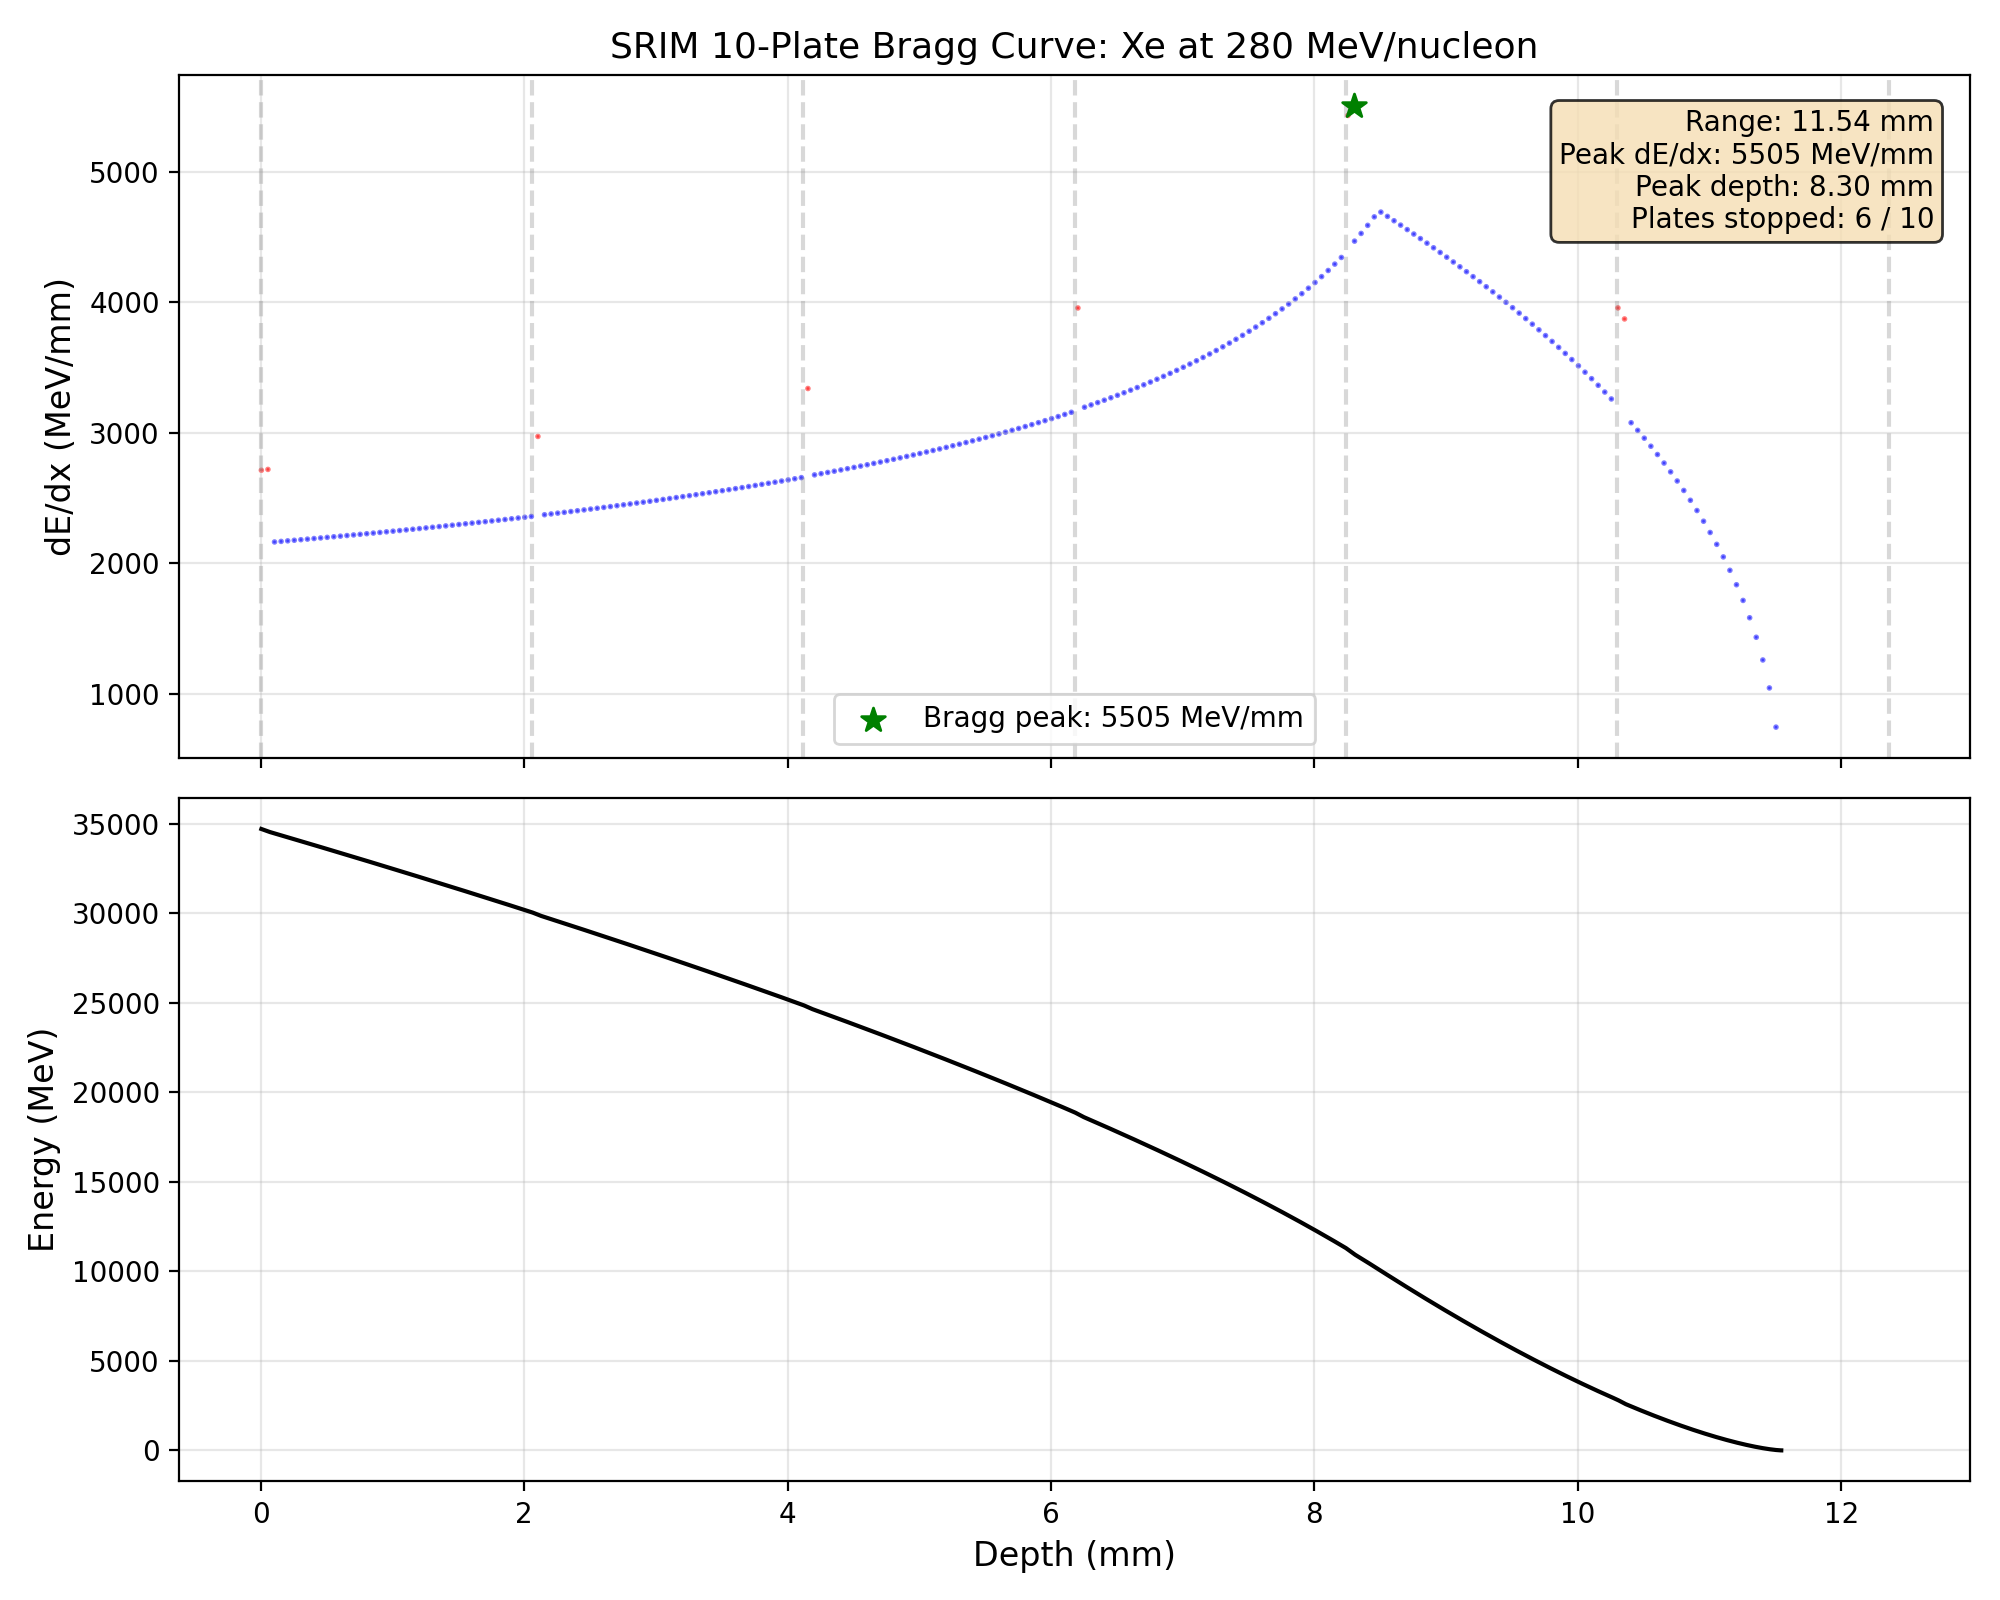
\includegraphics[width=0.90\textwidth]{srim_10plate_bragg.png}
\caption{SRIM-based 10-plate Bragg curve for
\textsuperscript{124}Xe at 280\,MeV/nucleon.
Top: $dE/dx$ vs.\ depth (red = emulsion, blue = glass).
Bottom: remaining kinetic energy vs.\ depth.
Dashed vertical lines mark the plate boundaries.}
\label{fig:srim_bragg}
\end{figure}

\subsection{Energy deposition per plate}

Table~\ref{tab:srim_energy} gives the energy budget for each plate.
Most of the beam energy is deposited in plates~2--5, with the maximum
per-plate loss ($\Delta E = 8467$\,MeV) in plate~5, where the Bragg
peak occurs. The ion stops during plate~6.

\begin{table}[H]
\centering
\caption{Energy deposition per plate from the SRIM simulation.}
\label{tab:srim_energy}
\begin{tabular}{crrrr}
\toprule
Plate & Depth range & $E_{\text{in}}$ & $\Delta E$ & $E_{\text{out}}$ \\
 & (mm) & (MeV) & (MeV) & (MeV) \\
\midrule
1 & 0.00--2.06 & 34720 & 4669 & 30051 \\
2 & 2.06--4.12 & 30051 & 5183 & 24868 \\
3 & 4.12--6.18 & 24868 & 5987 & 18882 \\
4 & 6.18--8.24 & 18882 & 7585 & 11297 \\
5 & 8.24--10.30 & 11297 & 8467 & 2831 \\
6 & 10.30--12.36 & 2831 & 2831 & 0 \\
7--10 & 12.36--20.60 & --- & --- & --- \\
\bottomrule
\end{tabular}
\end{table}

\subsection{Comparison with experiment}

Figure~\ref{fig:srim_vs_exp} compares the normalised SRIM-simulated
Bragg curve with the experimental energy deposition fraction
($\varepsilon_i$, Eq.~\ref{eq:edep}) from Stack\,03 (10 cycles, best
statistics). The SRIM curve is sampled at the plate centre positions
for direct comparison.

\begin{figure}[H]
\centering
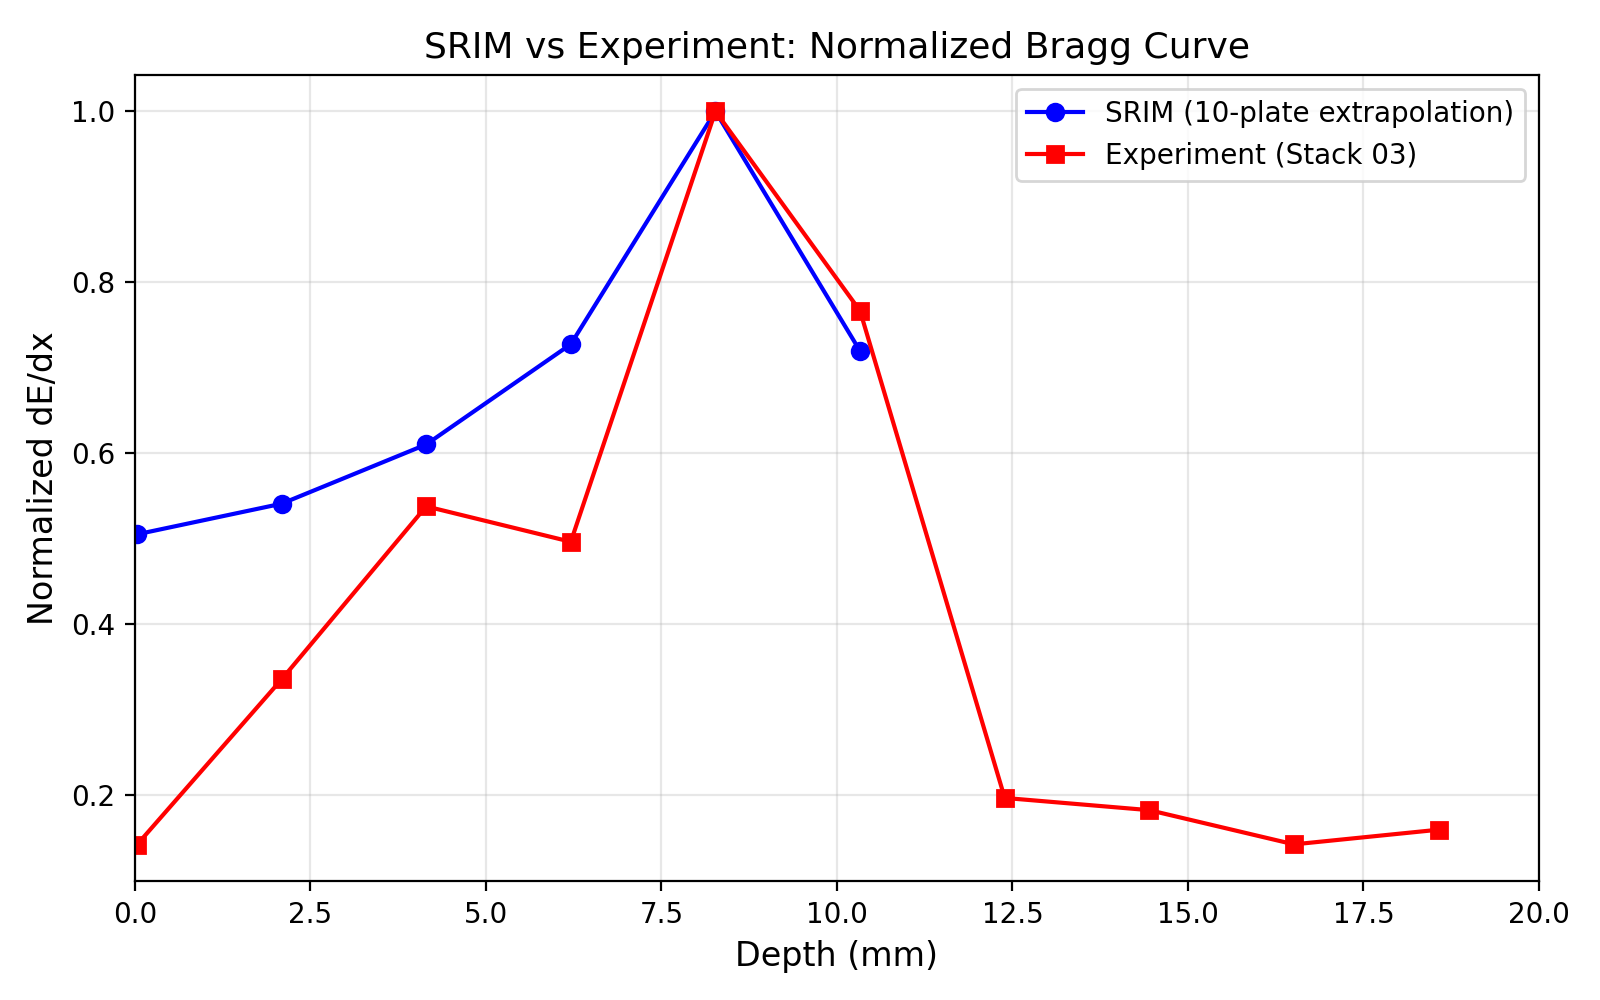
\includegraphics[width=0.75\textwidth]{srim_vs_exp.png}
\caption{Normalised Bragg curve: SRIM simulation vs.\ experiment
(Stack\,03). Both curves are normalised to their respective maxima.}
\label{fig:srim_vs_exp}
\end{figure}

The SRIM-predicted Bragg peak at 8--10\,mm is consistent with the
experimental observation of 10--12\,mm for Stack\,03. The agreement
in the rise slope (plates 1--5) supports the SRIM stopping power as
a valid model for this energy regime.

%===================================================================
\section{Olympus BX63 intelligent microscope}
\label{sec:microscope}
%===================================================================

Digital imaging of the emulsion plates was performed using an
\textbf{Olympus BX63} automated intelligent microscope.
The BX63 is a motorised upright microscope equipped with:

\begin{itemize}
  \item A motorised stage with computer-controlled X--Y--Z positioning
        for automated tiled scanning;
  \item A high-resolution digital CMOS camera;
  \item Multiple objective lenses (4$\times$, 20$\times$, 40$\times$);
  \item An LED illumination system for bright-field imaging;
  \item Olympus cellSens software for image acquisition and stitching.
\end{itemize}

\begin{figure}[H]
\centering
\begin{subfigure}{0.48\textwidth}
  \includegraphics[width=\textwidth]{jinr/microscope1.jpg}
  \caption{Olympus BX63 microscope overview.}
  \label{fig:micro1}
\end{subfigure}
\hfill
\begin{subfigure}{0.48\textwidth}
  \includegraphics[width=\textwidth]{jinr/microscope2.jpg}
  \caption{Microscope stage with emulsion plate mounted.}
  \label{fig:micro2}
\end{subfigure}

\begin{subfigure}{0.48\textwidth}
  \includegraphics[width=\textwidth]{jinr/microscope3.jpg}
  \caption{Close-up of the objective lens and stage.}
  \label{fig:micro3}
\end{subfigure}
\hfill
\begin{subfigure}{0.48\textwidth}
  \includegraphics[width=\textwidth]{jinr/microscope4.jpg}
  \caption{Computer interface for automated scanning.}
  \label{fig:micro4}
\end{subfigure}
\caption{Olympus BX63 intelligent microscope used for emulsion plate scanning.}
\label{fig:microscope}
\end{figure}

\begin{figure}[H]
\centering
\includegraphics[width=0.6\textwidth]{jinr/microscope_me.jpg}
\caption{Working with the Olympus BX63 microscope during plate scanning.}
\label{fig:micro_me}
\end{figure}

\subsection{Scanning procedure}

The microscope scans each plate in a raster pattern, acquiring several
thousand overlapping frames. The cellSens software stitches these
frames into a single high-resolution mosaic covering approximately 80\%
of the plate area. The total acquisition time per plate at 4$\times$
magnification is approximately 2--3 hours, depending on the scanned
area.

\subsection{Magnification choice}

Due to the high ionization density of the \textsuperscript{124}Xe beam
at 280\,MeV/nucleon, even the 4$\times$ objective (numerical aperture
NA = 0.10) produces sufficient contrast to resolve individual grain
clusters corresponding to particle tracks. This is confirmed by
comparison with 20$\times$ and 40$\times$ images (see
Sec.~\ref{sec:images}).

The pixel size at 4$\times$ magnification is approximately
1.717\,\si{\micro\meter}/pixel (Stack\,01), which provides adequate sampling
of grain sizes (typically 10--500\,\si{\micro\meter\squared}). For
Stacks\,02 and~03, the microscope software provided calibrated
micrometre coordinates directly, so the raw CSV values for area and
position are already in \si{\micro\meter} and \si{\micro\meter\squared}
respectively — no further pixel-to-micrometre conversion is needed.
This is confirmed by the Summary file headers
(e.g.\ \texttt{Avg\_Area\_um2}) and the \texttt{GeneratePlots.C} macro
which uses the raw \texttt{Area} and \texttt{XM}/\texttt{YM} values
directly.

\begin{figure}[H]
\centering
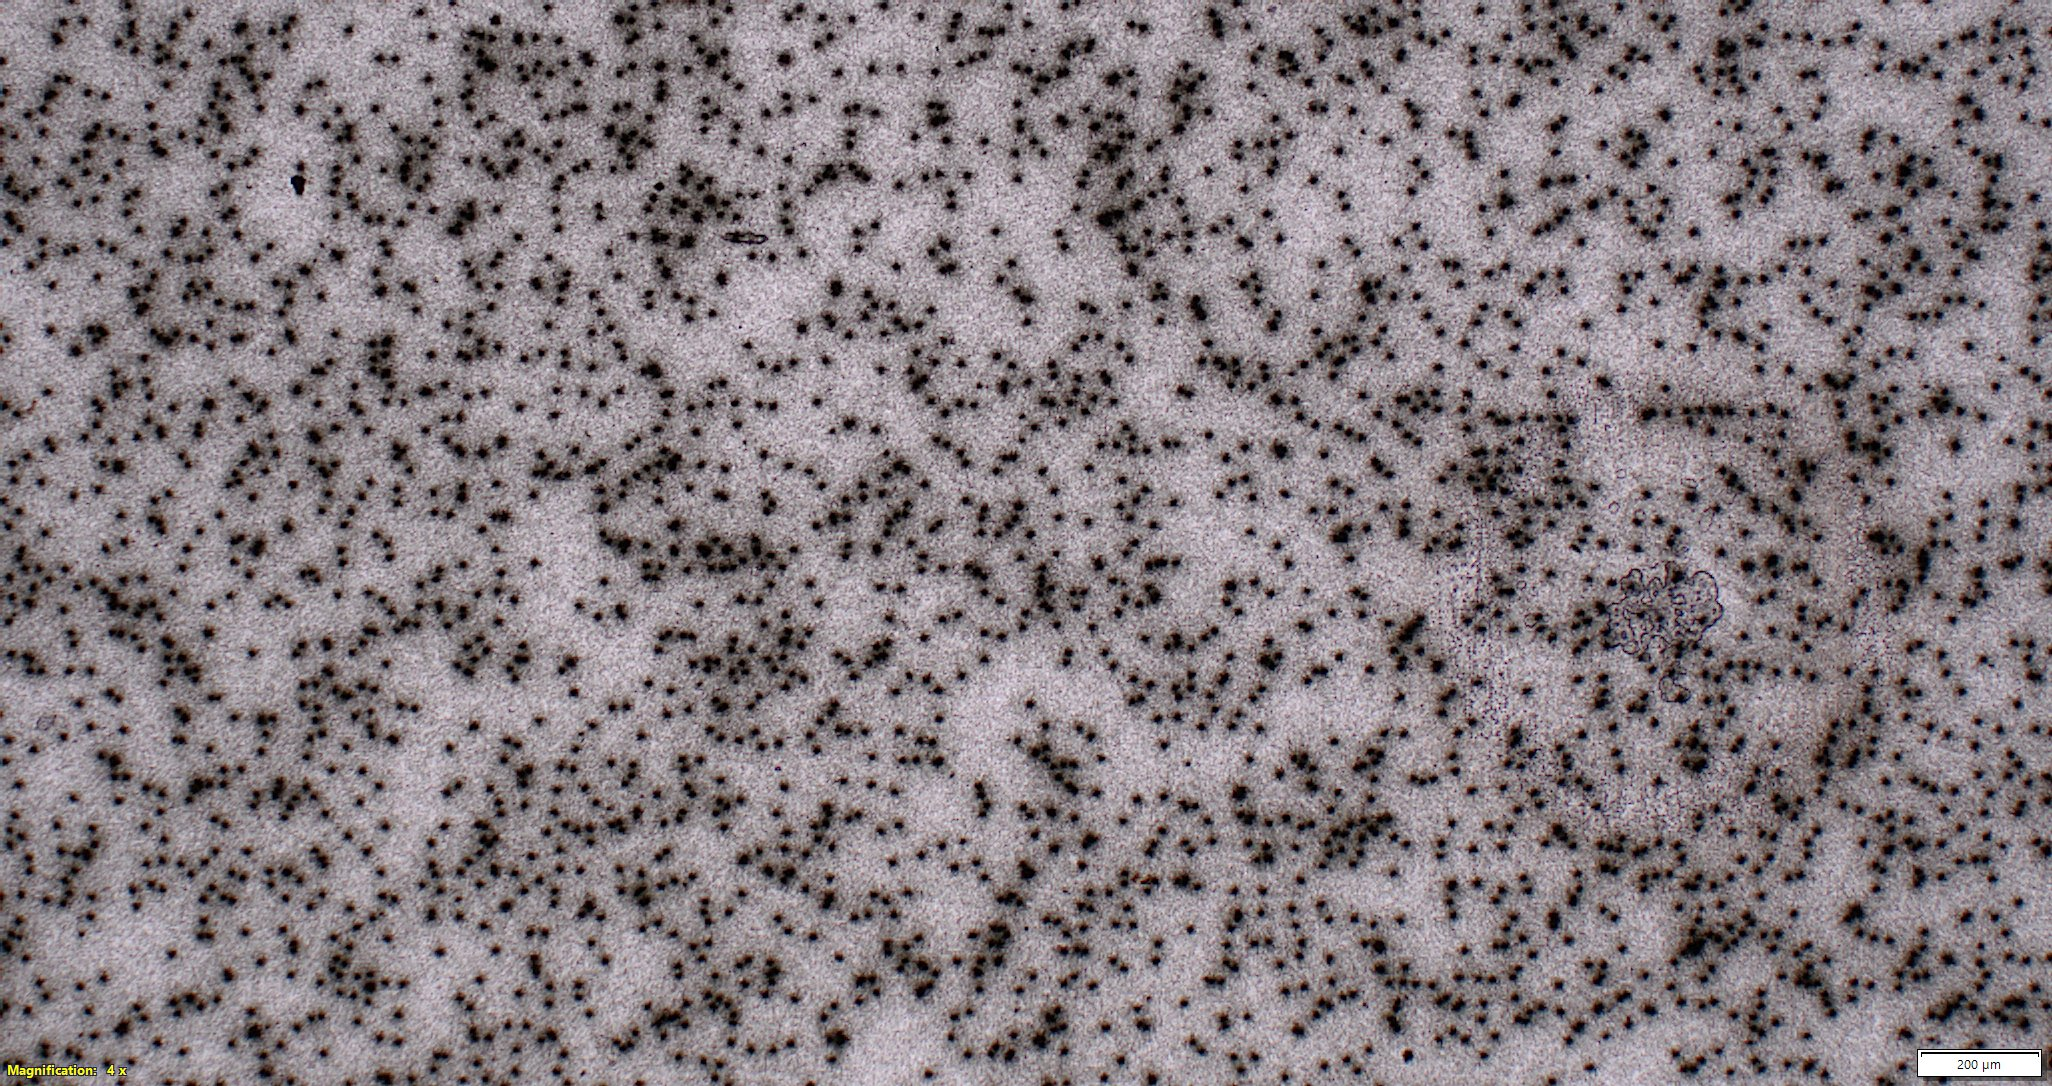
\includegraphics[width=0.65\textwidth]{../4x.jpg}
\caption{4$\times$ objective image of an emulsion plate showing the beam
spot region. Individual grain clusters from the Xe beam and its
fragments are visible as dark features against the lighter emulsion
background.}
\label{fig:4x}
\end{figure}

%===================================================================
\section{ImageJ software}
\label{sec:imagej}
%===================================================================

ImageJ~\cite{imagej} is an open-source, Java-based image processing
package developed at the National Institutes of Health (NIH). It was
used for all grain detection and measurement tasks in this work.

\subsection{Key features used}

The following ImageJ functions were employed in the analysis pipeline:

\begin{description}
  \item[Set Scale:] Calibration of pixel-to-micrometre conversion.
        For Stack\,01, the scale was set to 1.717\,\si{\micro\meter}/pixel (determined from
        a stage micrometre image), so the raw CSV values are in pixel
        units and must be divided by $1.717^2$ to obtain
        \si{\micro\meter\squared} for area. For Stacks\,02 and~03, the
        microscope software already provided calibrated images, so the
        raw \texttt{Area}, \texttt{XM}, and \texttt{YM} columns are
        directly in \si{\micro\meter\squared} and \si{\micro\meter}.  
  \item[Enhance Contrast:] Normalises the image histogram by saturating
        0.35\% of pixels, reducing the effect of illumination gradients
        across the stitched mosaic.
  \item[Threshold:] A fixed threshold of 0--75 on the 8-bit greyscale
        image (0 = black, 255 = white) converts the image to a binary
        mask. This range was chosen empirically: developed silver
        grains appear dark (pixel values 0--75), while the clear
        emulsion background is bright (typical pixel value $\sim$180).
  \item[Convert to Mask:] Creates a binary image from the threshold.
  \item[Analyze Particles:] Identifies connected pixel clusters and
        measures their morphological parameters.
\end{description}

\subsection{Particle analysis parameters}

The particle analysis filter was configured with:
\begin{itemize}
  \item Size range: 10--1200\,px\textsuperscript{2}
        (approximately 3.4--410\,\si{\micro\meter\squared}
        at 1.717\,\si{\micro\meter}/pixel);
  \item Circularity: 0.00--1.00 (no restriction);
  \item Output: ``Nothing'' (no outlines), with measurement results
        saved to a table.
\end{itemize}

\subsection{Batch processing macros}

Dedicated ImageJ macros were written for automated batch processing:

\begin{itemize}
  \item \texttt{Emulsion\_Analysis.C} (Stack\,01): processes all 8
        plates, saves per-plate Results CSV and Summary CSV;
  \item \texttt{Macro2.ijm} (Stack\,02): same pipeline for 10 plates,
        with skip logic to avoid reprocessing existing files;
  \item \texttt{Macro3.ijm} (Stack\,03): same pipeline for 10 plates.
\end{itemize}

All macros iterate over all TIFF files in the \texttt{Emulsion\_Files}
directory, perform the detection pipeline, and write both the
individual plate Results CSV and a summary file with statistics
(count, total area, average area, roundness, solidity, etc.).

%===================================================================
\section{Images at 4$\times$, 20$\times$, 40$\times$}
\label{sec:images}
%===================================================================

To verify that the 4$\times$ magnification is adequate for track
detection, comparative images were taken at 4$\times$, 20$\times$,
and 40$\times$ magnifications.

\begin{figure}[H]
\centering
\begin{subfigure}{0.32\textwidth}
  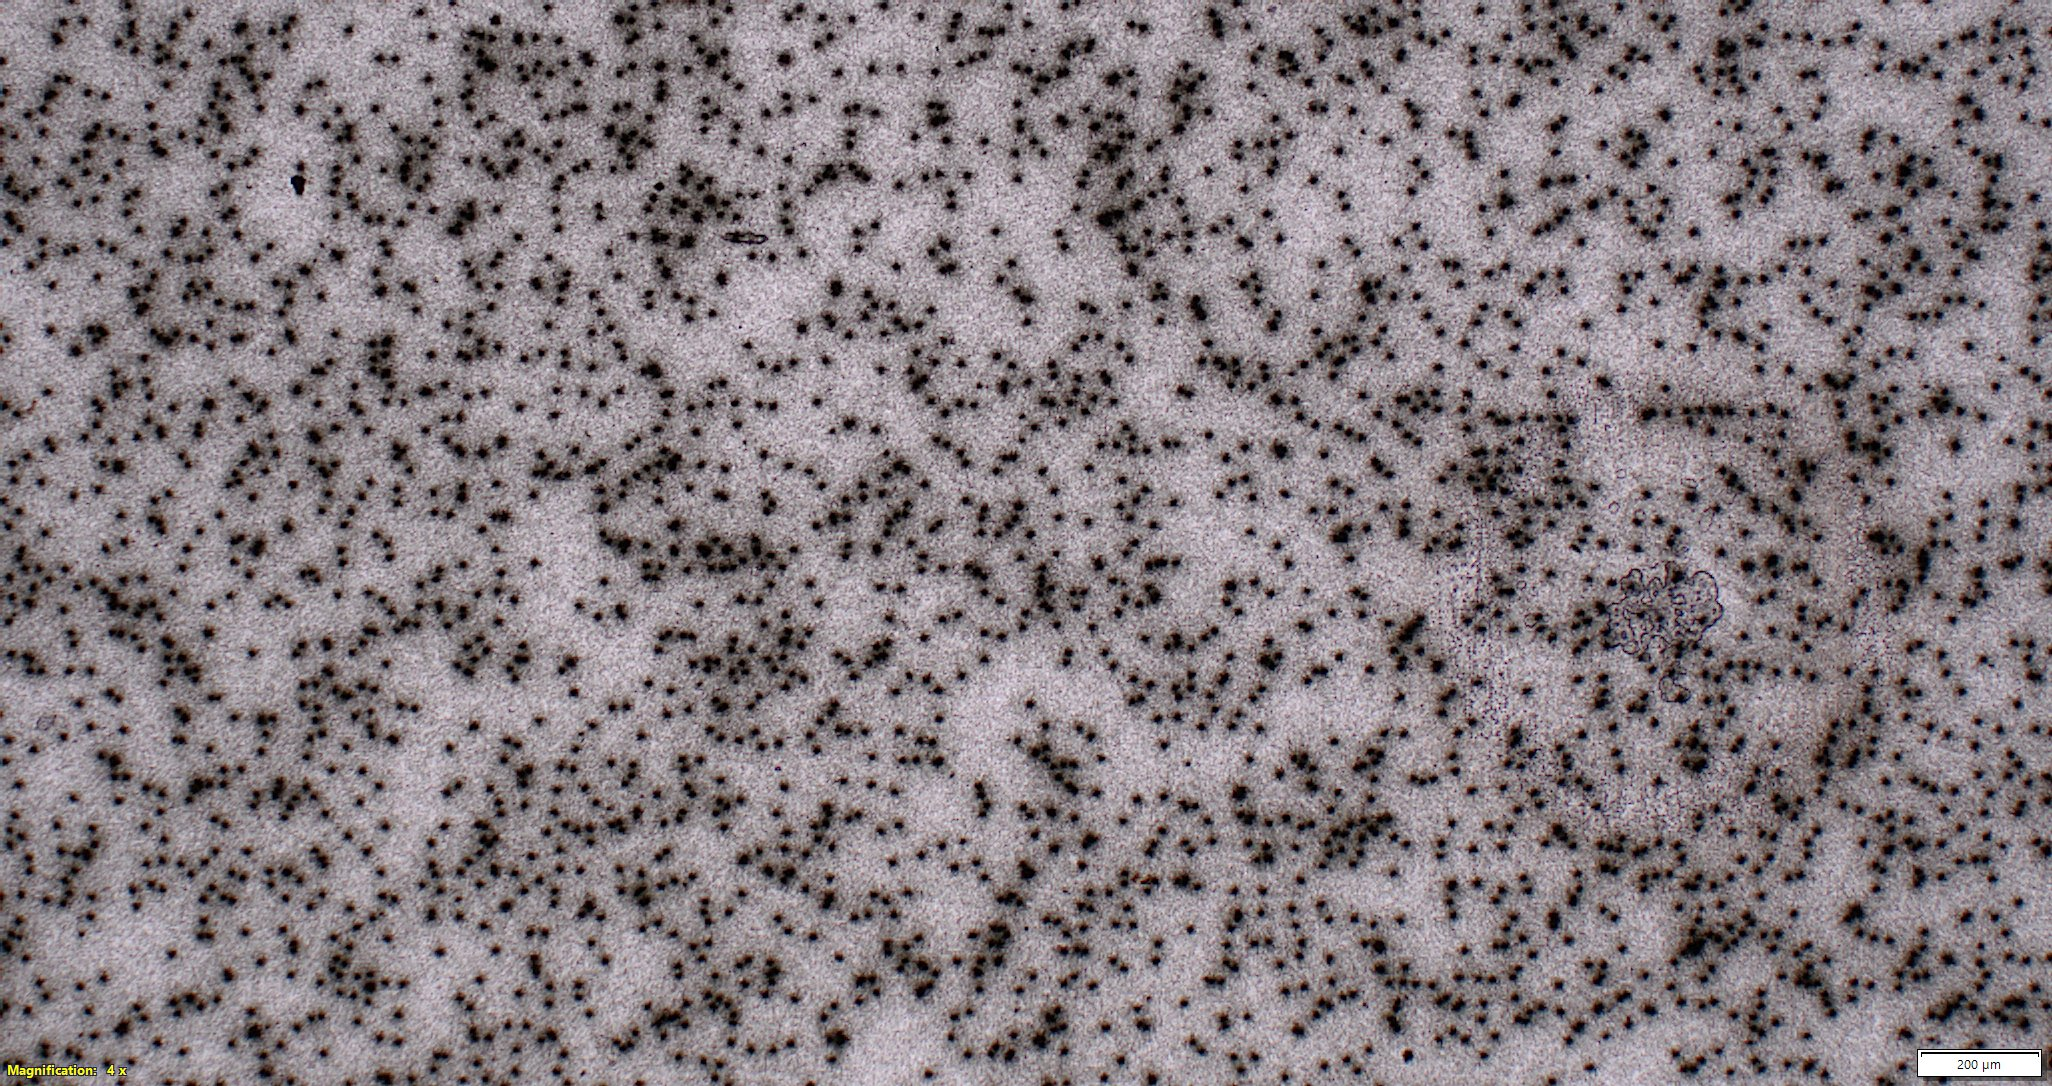
\includegraphics[width=\textwidth,height=0.2\textheight,keepaspectratio]{../4x.jpg}
  \caption{4$\times$ objective. Field of view
  $\sim$2$\times$1.5\,mm. Grain clusters are visible as dark
  features. Scale bar $\sim$125\,\si{\micro\meter}.}
  \label{fig:4x_detail}
\end{subfigure}
\hfill
\begin{subfigure}{0.32\textwidth}
  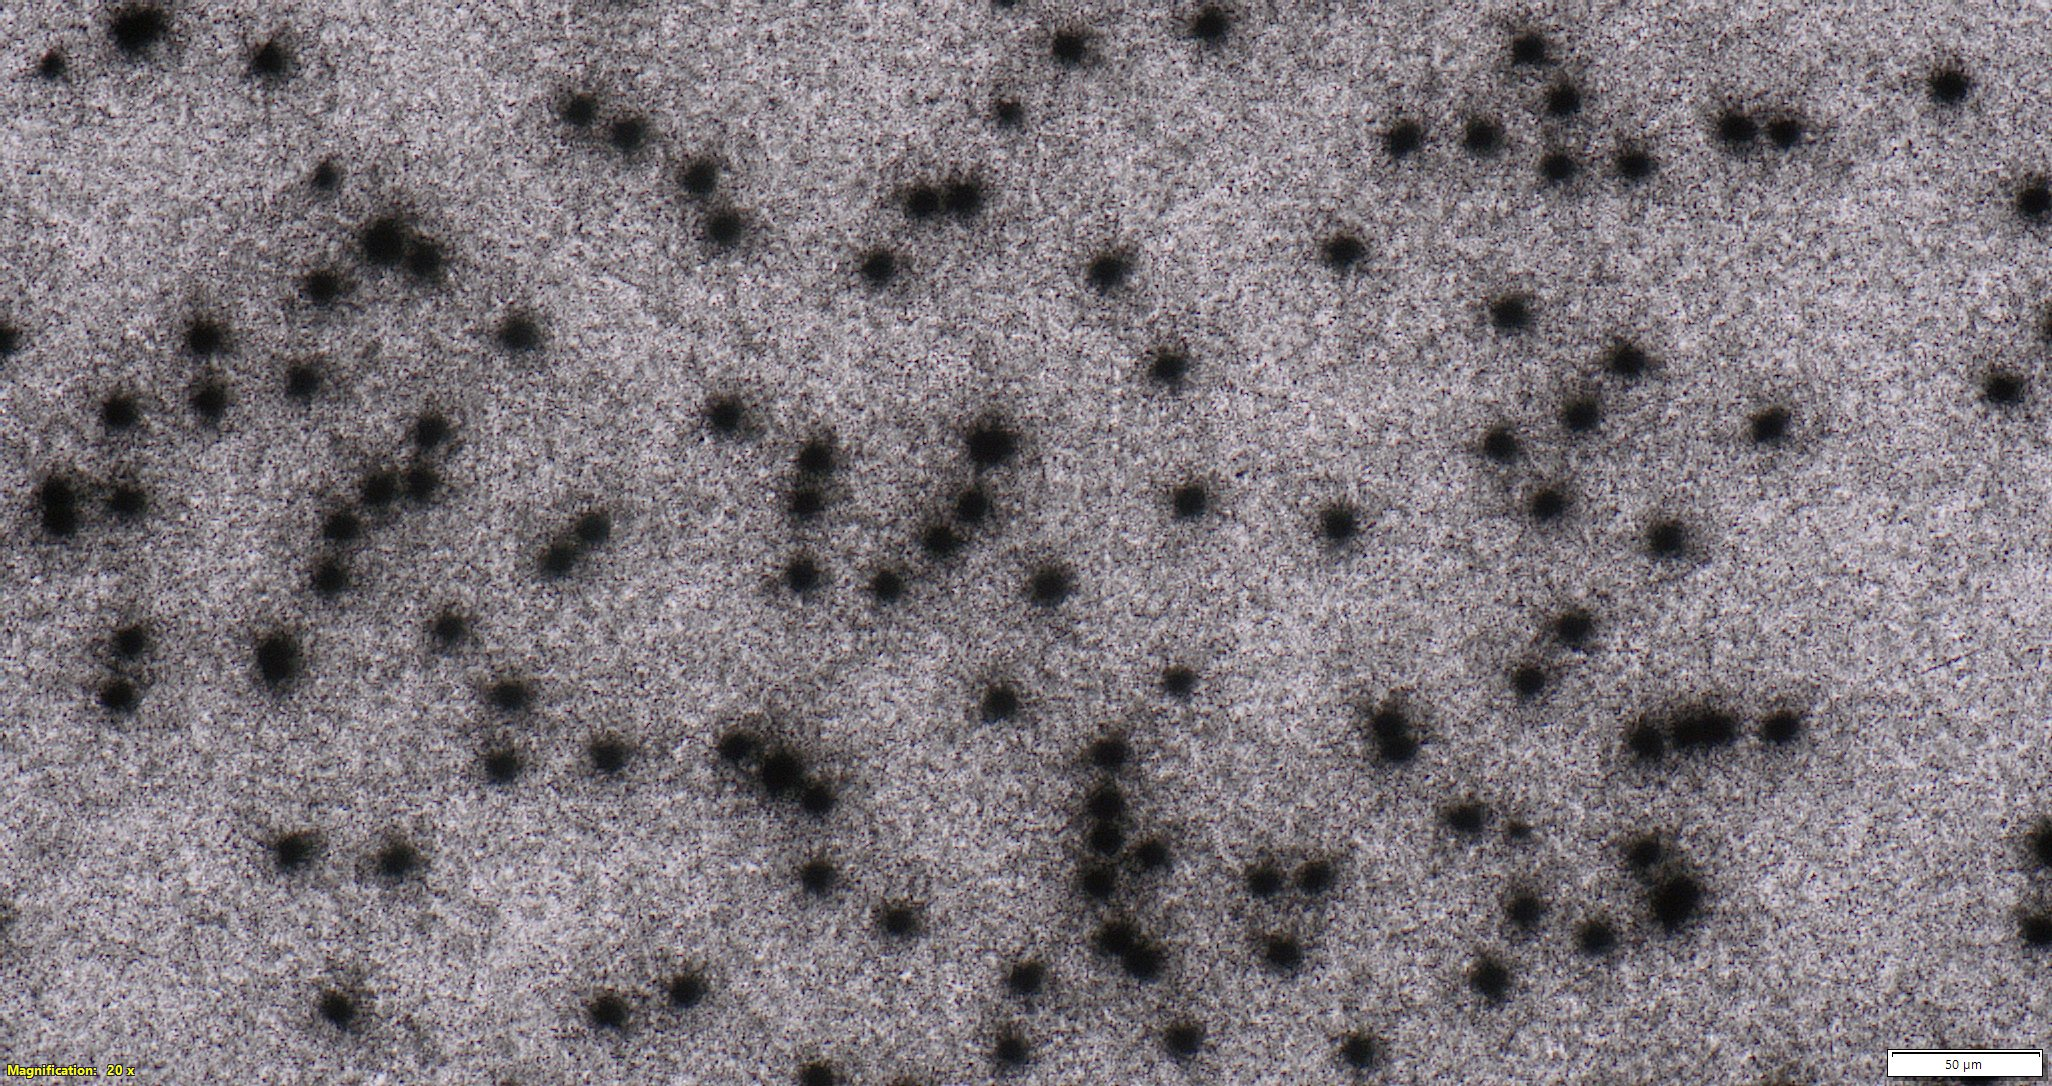
\includegraphics[width=\textwidth,height=0.2\textheight,keepaspectratio]{../20x.jpg}
  \caption{20$\times$ objective. Individual grains begin to be
  resolved. Scale bar $\sim$25\,\si{\micro\meter}.}
  \label{fig:20x}
\end{subfigure}
\hfill
\begin{subfigure}{0.32\textwidth}
  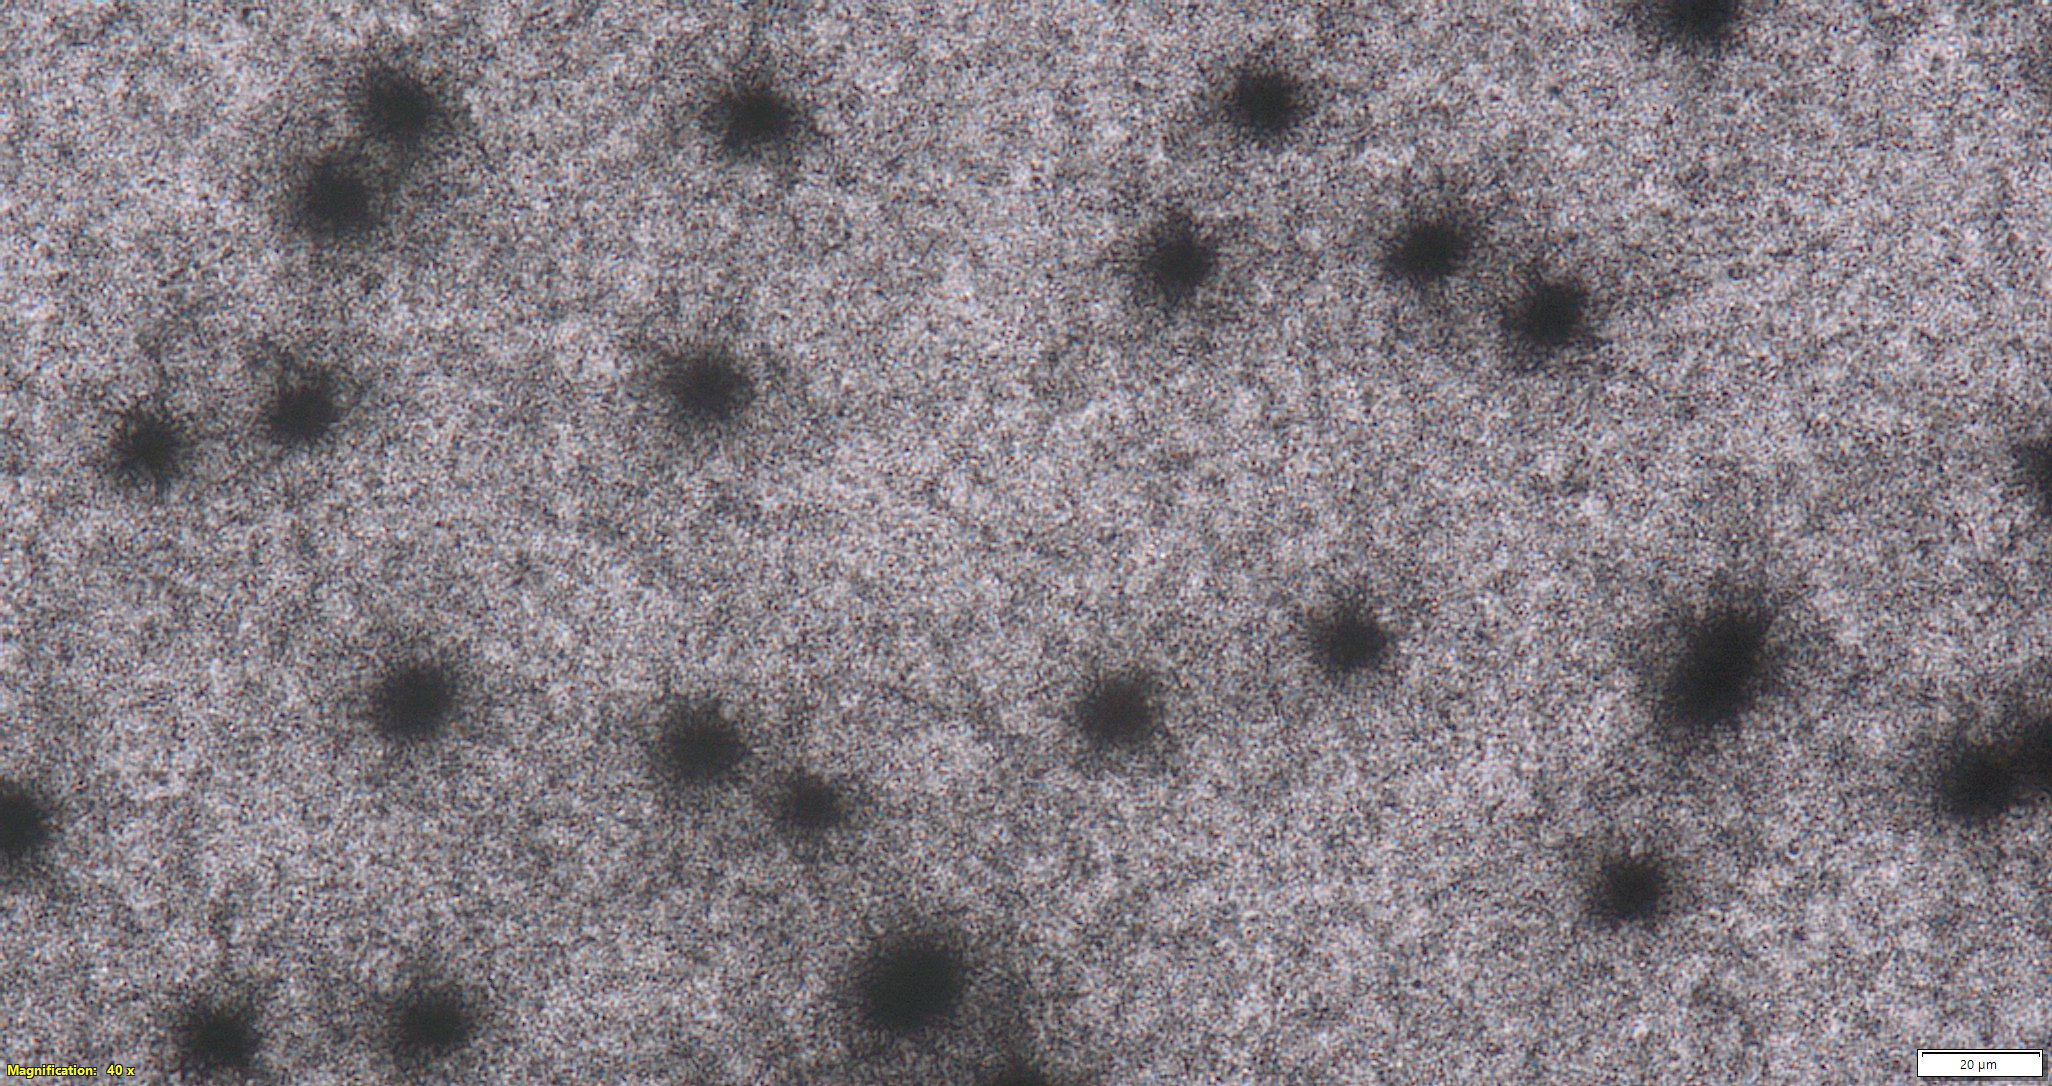
\includegraphics[width=\textwidth,height=0.2\textheight,keepaspectratio]{../40x.jpg}
  \caption{40$\times$ objective. Individual silver grains are
  clearly resolved. Scale bar $\sim$12\,\si{\micro\meter}.}
  \label{fig:40x}
\end{subfigure}
\caption{Comparison of the same emulsion region at three
magnifications. At 4$\times$ the grain clusters are detectable without
resolving individual grains; at 40$\times$ the internal structure of
each track is visible. The 4$\times$ objective provides sufficient
sensitivity for counting and area measurement.}
\label{fig:mag_compare}
\end{figure}

At 4$\times$ magnification, individual particle tracks appear as small
dark clusters of merged grains against the lighter emulsion background.
The field of view is approximately $2\times1.5$\,mm, allowing rapid
scanning of large plate areas. The grain shapes range from nearly
circular (roundness $>0.8$) for small, isolated grains to irregular,
fragmented shapes for heavily ionising tracks where adjacent grains
merge.

At 40$\times$ magnification, the internal structure of individual grain
clusters becomes visible, confirming that the 4$\times$ detection is
counting clusters of multiple silver grains rather than individual
grains. This is expected and acceptable: the cluster area is
proportional to the energy deposition of the parent particle.

The decision to use 4$\times$ for the full plate scan represents an
optimal trade-off between resolution and throughput: it is sufficient to
detect all tracks from the Xe beam and its fragments, while keeping the
total acquisition time per plate manageable.

%===================================================================
\section{Image recognition in ImageJ}
\label{sec:recognition}
%===================================================================

\subsection{Processing pipeline}

The automated grain detection pipeline for each plate follows these
steps:

\begin{enumerate}
  \item \textbf{Image acquisition:} The stitched TIFF mosaic from the
        Olympus cellSens software is loaded into ImageJ. Typical
        image dimensions are 40,000--60,000 pixels per side.
  \item \textbf{Scale calibration:} The pixel-to-micrometre conversion
        is set. For Stack\,01: \texttt{Set Scale... distance=1.717
        known=1 pixel=1 unit=um}. For Stacks\,02 and~03, the images \\
        are already calibrated.
  \item \textbf{Contrast enhancement:} \texttt{Enhance Contrast
        saturated=0.35 normalize} normalises the histogram.
  \item \textbf{Thresholding:} \texttt{setThreshold(0, 75)} creates
        a binary mask where dark pixels (grains) are selected.
  \item \textbf{Convert to Mask:} Converts the threshold to a binary
        image.
  \item \textbf{Particle analysis:} \texttt{Analyze Particles
        size=10-1200 circularity=0.00-1.00 \\ show=Nothing display
        exclude include add} detects all connected components.
  \item \textbf{Result export:} Measurements are saved as CSV files.
\end{enumerate}

\subsection{Measured parameters}

For each detected grain cluster, the following parameters are
recorded:

\begin{itemize}
  \item \textbf{Area} (\si{\micro\meter\squared}): Projected area of the
        grain cluster.
  \item \textbf{Perimeter} (\si{\micro\meter}): Length of the cluster
        boundary.
  \item \textbf{Feret diameter} (\si{\micro\meter}): Maximum caliper
        length (longest axis).
  \item \textbf{FeretX, FeretY} (\si{\micro\meter}): Coordinates of the
        centroid.
  \item \textbf{Circularity}: $4\pi A/P^2$, where $A$ is area and $P$
        is perimeter. A perfect circle has circularity $= 1.0$.
  \item \textbf{Roundness}: $4A/(\pi F^2)$, where $F$ is the Feret
        diameter.
  \item \textbf{Solidity}: $A / A_{\text{convex}}$, the ratio of the
        area to its convex hull area.
\end{itemize}

\subsection{Example: single-plate analysis}

An early analysis of one plate (from the preliminary study) detected
396 particles in a single field of view at 4$\times$ magnification.
The mean grain area was 272\,px\textsuperscript{2}
($\sim$92\,\si{\micro\meter\squared}), mean Feret diameter 24\,px
($\sim$14\,\si{\micro\meter}), and mean circularity 0.83, confirming that the
majority of detected objects are compact, approximately circular grain
clusters.

%===================================================================
\section{Image parameters by layer}
\label{sec:params}
%===================================================================

\subsection{Summary statistics per plate}

For each plate, the following parameters were computed from the grain
measurements:

\begin{align}
\text{Track density:}\quad &
\rho_i = \frac{N_i}{A_i}, \quad
A_i = (\max x_i - \min x_i)(\max y_i - \min y_i), \label{eq:density}\\
\text{Mean grain area:}\quad &
\bar{a}_i = \frac{1}{N_i}\sum_{j=1}^{N_i} a_{ij}, \label{eq:meanarea}\\
\text{Energy deposition fraction:}\quad &
\varepsilon_i = \frac{1}{A_i}\sum_{j=1}^{N_i} a_{ij}. \label{eq:edep}
\end{align}

The energy deposition fraction $\varepsilon_i$ (Eq.~\ref{eq:edep}) is a
proxy for the specific energy loss $dE/dx$: it represents the
fraction of the scanned area that is covered by developed silver
grains.

\noindent\textbf{Scanner calibration note.}
The three stacks were scanned with different calibration modes:
Stack\,01 raw CSV values are in pixel units (scale
1.717\,\si{\micro\meter}/pixel), so the analysis script divides
\texttt{Area} by $1.717^2$ and \texttt{FeretX}/\texttt{FeretY} by
1.717 to obtain micrometre units.
Stacks\,02 and~03 were already saved in calibrated micrometre units by
the microscope software (\texttt{XM}, \texttt{YM} columns), so no
pixel-to-micrometre conversion is applied.
The \texttt{GeneratePlots.C} macro for Stack\,02 confirms this: it
uses the raw \texttt{Area} and coordinate values directly with no
scaling factor (the TIFF pixel dimensions are converted with 1.717
\emph{only} for display of the plate extent).

\subsection{Per-plate data tables}

Full per-plate results for all three stacks are given in
Table~\ref{tab:bragg_full}. The data are also available as CSV files
(\texttt{bragg\_data.csv}).

\begin{table}[H]
\centering
\caption{Full Bragg curve data for all three stacks.}
\label{tab:bragg_full}
\begin{tabular}{crrrrrr}
\toprule
Stack & Plate & Depth & $N_{\text{grains}}$ & Scan area &
$\rho$ & $\bar{a}$ \\
 & & (mm) & & (\si{\mm\squared}) &
(\si{\mm^{-2}}) & (\si{\micro\meter\squared}) \\
\midrule
\multicolumn{7}{c}{\textbf{Stack\,01 (1 cycle)}} \\
\rule{0pt}{2ex}
1 & 1\_Plate\_09 & 0.03 & 245,858 & 406.5 & 605 & 82.2 \\
1 & 2\_Plate\_08 & 2.09 & 216,951 & 442.6 & 490 & 115.9 \\
1 & 3\_Plate\_07 & 4.15 & 244,781 & 469.7 & 521 & 87.3 \\
1 & 4\_Plate\_06 & 6.21 & 197,686 & 469.1 & 421 & 128.0 \\
1 & 5\_Plate\_05 & 8.27 & 227,371 & 471.5 & 482 & 124.6 \\
1 & 6\_Plate\_04 & 10.33 & 16,091 & 470.8 & 34 & 51.0 \\
1 & 7\_Plate\_03 & 12.39 & 13,421 & 469.7 & 29 & 43.8 \\
1 & 8\_Plate\_02 & 14.45 & 5,787 & 470.1 & 12 & 67.5 \\
\midrule
\multicolumn{7}{c}{\textbf{Stack\,02 (5 cycles)}} \\
\rule{0pt}{2ex}
2 & 1\_Plate-0001 & 0.03 & 429,943 & 457.7 & 939 & 44.6 \\
2 & 2\_Plate-0001 & 2.09 & 504,675 & 3975.8 & 127 & 192.4 \\
2 & 3\_Plate-0001 & 4.15 & 492,439 & 3957.6 & 124 & 279.2 \\
2 & 4\_Plate-0001 & 6.21 & 498,347 & 3977.3 & 125 & 268.7 \\
2 & 5\_Plate-0001 & 8.27 & 506,437 & 3962.2 & 128 & 287.9 \\
2 & 6\_Plate-0001 & 10.33 & 488,378 & 3591.2 & 136 & 329.9 \\
2 & 7\_Plate-0001 & 12.39 & 137,362 & 3582.7 & 38 & 70.6 \\
2 & 8\_Plate-0001 & 14.45 & 121,953 & 3582.6 & 34 & 75.6 \\
2 & 9\_Plate-0001 & 16.51 & 306,163 & 3582.9 & 85 & 37.7 \\
2 & 10\_Plate\_001 & 18.57 & 24,955 & 413.2 & 60 & 32.0 \\
\midrule
\multicolumn{7}{c}{\textbf{Stack\,03 (10 cycles)}} \\
\rule{0pt}{2ex}
3 & Plate\_01\_p1 & 0.03 & 1,089,177 & 440.0 & 2475 & 29.6 \\
3 & Plate\_02\_p1 & 2.09 & 1,174,887 & 1301.9 & 902 & 70.2 \\
3 & Plate\_03\_p1 & 4.15 & 1,037,403 & 1301.7 & 766 & 112.7 \\
3 & Plate\_04\_p1 & 6.21 & 1,048,569 & 1301.6 & 806 & 104.0 \\
3 & Plate\_05\_p1 & 8.27 & 1,075,283 & 1302.5 & 633 & 209.7 \\
3 & Plate\_06\_p1 & 10.33 & 1,169,823 & 1345.5 & 680 & 160.7 \\
3 & Plate\_07\_p1 & 12.39 & 60,014 & 1343.5 & 45 & 41.1 \\
3 & Plate\_08\_p1 & 14.45 & 56,852 & 1347.9 & 42 & 38.1 \\
3 & Plate\_09\_p1 & 16.51 & 34,492 & 1215.2 & 28 & 29.7 \\
3 & Plate\_10\_p1 & 18.57 & 26,061 & 1214.9 & 21 & 33.3 \\
\bottomrule
\end{tabular}
\end{table}

\subsection{Summary statistics}

The Summary CSV files per plate provide additional morphological
parameters. For Stack\,02, which has the most complete data:

\begin{table}[H]
\centering
\caption{Morphological summary for Stack\,02 plates.}
\label{tab:morph}
\begin{tabular}{crrrrrc}
\toprule
Plate & $N$ & Avg area & Avg roundness & Avg solidity &
Avg perimeter \\
 & & (\si{\micro\meter\squared}) & & & (\si{\micro\meter}) \\
\midrule
1\_Plate-0001 & 429,943 & 44.6 & 0.801 & 0.784 & --- \\
2\_Plate-0001 & 504,675 & 192.4 & 0.693 & 0.832 & --- \\
3\_Plate-0001 & 492,439 & 279.2 & 0.668 & 0.846 & --- \\
4\_Plate-0001 & 498,347 & 268.7 & 0.684 & 0.838 & --- \\
5\_Plate-0001 & 506,437 & 287.9 & 0.674 & 0.841 & --- \\
6\_Plate-0001 & 488,378 & 329.9 & 0.662 & 0.845 & --- \\
7\_Plate-0001 & 137,362 & 70.6 & 0.550 & 0.743 & --- \\
8\_Plate-0001 & 121,953 & 75.6 & 0.547 & 0.742 & --- \\
9\_Plate-0001 & 306,163 & 37.7 & 0.064 & 0.633 & --- \\
10\_Plate\_001 & 24,955 & 32.0 & 0.631 & 0.736 & --- \\
\bottomrule
\end{tabular}
\end{table}

The roundness and solidity decrease after the Bragg peak (plates 7+),
indicating that the surviving light fragments produce more irregular,
fragmented grain clusters.

%===================================================================
\section{Input area distribution. Uniformity}
\label{sec:uniformity}
%===================================================================

\subsection{Grain area distribution}

The grain area distribution in each plate follows a multi-modal pattern,
reflecting the superposition of particles with different ionization
densities. The distribution is approximately log-normal for each
sub-population. Figure~\ref{fig:classes} shows the three components
identified by the Gaussian Mixture Model (see Sec.~\ref{sec:gmm}).

\begin{figure}[H]
\centering
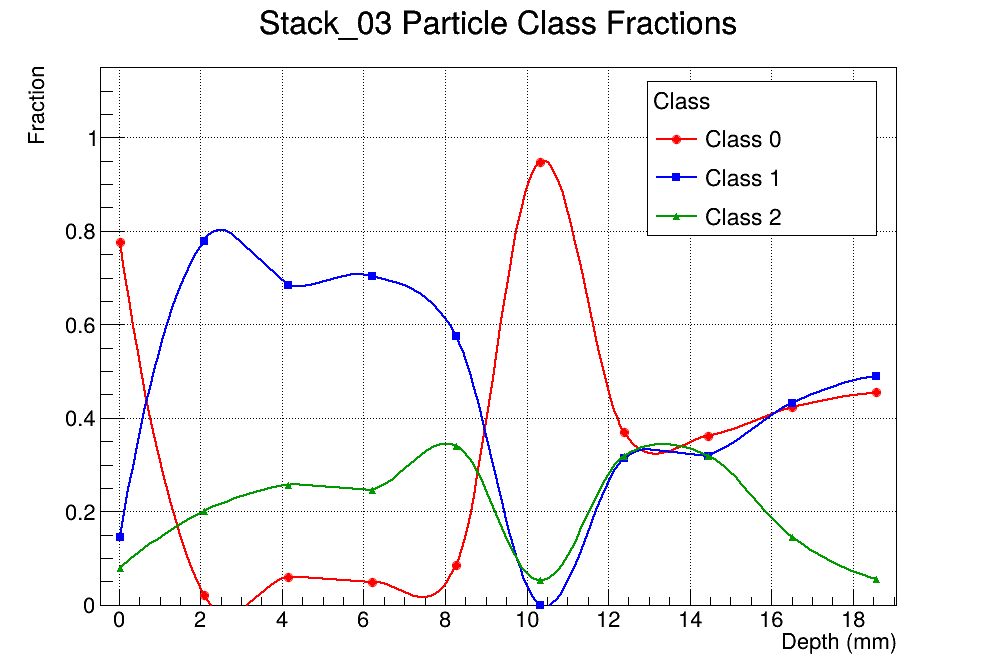
\includegraphics[width=0.75\textwidth]{./Stack_03_particle_classes.png}
\caption{Particle class fractions vs.\ depth for Stack\,03.
Class 0 = smallest grains (light fragments, MIPs);
Class 1 = medium grains (mid-Z fragments);
Class 2 = largest grains (primary Xe beam, heavy fragments).
The uncertainty in class fractions is statistical only.}
\label{fig:classes}
\end{figure}

\subsection{Beam profile uniformity}

The lateral beam profile was assessed using the spatial distribution
of grains in each plate. A full set of 13 diagnostic plots was
generated per plate using the ROOT macro \texttt{GeneratePlots.C}.
Figures~\ref{fig:area}-\ref{fig:xyprof} show the complete set for
Stack\,02, Plate\,1 (1\_Plate-0001), which is the entrance plate with
the highest statistical sample (429,943 grains).

\begin{figure}[H]
\centering
\begin{subfigure}{0.48\textwidth}
  
\includegraphics[width=\textwidth]{../Stack_02/Plots/1_Plate-0001/02_AreaDistribution.png}
  \caption{\textbf{02\_AreaDistribution.png} -- Grain area histogram.
  Shows the distribution of individual grain areas in
  \si{\micro\meter\squared}. The distribution is strongly peaked at
  small areas ($\sim$10--50\,\si{\micro\meter\squared}) with a long
  tail extending to $>$1000\,\si{\micro\meter\squared}. The shape
  reflects the superposition of multiple particle populations with
  different $dE/dx$.}
  \label{fig:area}
\end{subfigure}
\hfill
\begin{subfigure}{0.48\textwidth}
  
\includegraphics[width=\textwidth]{../Stack_02/Plots/1_Plate-0001/03_FeretDistribution.png}
  \caption{\textbf{03\_FeretDistribution.png} -- Effective diameter
  distribution. The Feret (maximum caliper) diameter is approximated as
  $d_{\text{eff}} = 2\sqrt{A/\pi}$, the diameter of a circle of
  equivalent area. The peak at $\sim$5--10\,\si{\micro\meter}
  corresponds to the typical grain size.}
  \label{fig:feret}
\end{subfigure}
\end{figure}

\begin{figure}[H]
\centering
\begin{subfigure}{0.48\textwidth}
  
\includegraphics[width=\textwidth]{../Stack_02/Plots/1_Plate-0001/04_CircularityRoundness.png}
  \caption{\textbf{04\_CircularityRoundness.png} -- Two-panel histogram
  of circularity (left) and roundness (right). Circularity
  $= 4\pi A/P^2$; a perfect circle has value 1. Roundness
  $= 4A/(\pi F^2)$. Most grains have circularity $>0.6$ and roundness
  $>0.7$, confirming that the detected objects are compact grain
  clusters rather than irregular debris.}
  \label{fig:circround}
\end{subfigure}
\hfill
\begin{subfigure}{0.48\textwidth}
  
\includegraphics[width=\textwidth]{../Stack_02/Plots/1_Plate-0001/05_2DDensityHeatmap.png}
  \caption{\textbf{05\_2DDensityHeatmap.png} -- 2D density heatmap of
  grain positions across the full scanned area. The colour scale
  represents the number of grains per bin. This plot reveals the
  spatial distribution of the beam: a central concentration with a
  gradual radial fall-off, consistent with a Gaussian beam profile.
  The rectangular boundaries reflect the scanned region.}
  \label{fig:2dheat}
\end{subfigure}
\end{figure}

\begin{figure}[H]
\centering
\begin{subfigure}{0.48\textwidth}
  
\includegraphics[width=\textwidth]{../Stack_02/Plots/1_Plate-0001/06_2DScatterPlot.png}
  \caption{\textbf{06\_2DScatterPlot.png} -- 2D scatter plot of all
  individual grain positions (each dot is one grain). The density of
  points is highest at the centre and decreases radially. The
  approximately circular symmetry confirms that the beam was well
  centred on the plate and had no major hot spots or shadows.}
  \label{fig:2dscat}
\end{subfigure}
\hfill
\begin{subfigure}{0.48\textwidth}
  
\includegraphics[width=\textwidth]{../Stack_02/Plots/1_Plate-0001/07_RadialDensityProfile.png}
  \caption{\textbf{07\_RadialDensityProfile.png} -- Radial density
  profile. Grain density (count per \si{\micro\meter\squared}) is
  plotted as a function of radial distance from the beam centre. The
  density is maximum at $r=0$ and decreases monotonically, following a
  Gaussian-like distribution. The width (HWHM $\sim$5--8\,mm)
  characterises the beam spot size.}
  \label{fig:radprof}
\end{subfigure}
\end{figure}

\begin{figure}[H]
\centering
\begin{subfigure}{0.48\textwidth}
  
\includegraphics[width=\textwidth]{../Stack_02/Plots/1_Plate-0001/08_DifferentialFlux.png}
  \caption{\textbf{08\_DifferentialFlux.png} -- Differential flux
  $dN/dA$ as a function of grain area. This is the area distribution
  normalised by bin width. The peak at small areas corresponds to the
  most abundant grain population (minimum-ionising particles and
  light fragments).}
  \label{fig:dflux}
\end{subfigure}
\hfill
\begin{subfigure}{0.48\textwidth}
  
\includegraphics[width=\textwidth]{../Stack_02/Plots/1_Plate-0001/09_CumulativeCount.png}
  \caption{\textbf{09\_CumulativeCount.png} -- Cumulative distribution
  of grain areas. Shows what percentage of grains have area less than
  a given value. For example, $\sim$90\% of grains have area
  $<100$\,\si{\micro\meter\squared}, and $\sim$50\% have area
  $<30$\,\si{\micro\meter\squared}. The gradual rise reflects the
  broad dynamic range of grain sizes.}
  \label{fig:cumul}
\end{subfigure}
\end{figure}

\begin{figure}[H]
\centering

\includegraphics[width=0.75\textwidth]{../Stack_02/Plots/1_Plate-0001/10_LocalFluenceMap.png}
\caption{\textbf{10\_LocalFluenceMap.png} -- Local fluence map.
The scanned area is divided into a $10\times10$ grid and the grain
count per cell is displayed as both colour and text. This provides a
quantitative view of the fluence uniformity: the central cells have
the highest counts, with a smooth gradient to the edges. No anomalous
cell values are observed.}
\label{fig:fluence}
\end{figure}

\begin{figure}[H]
\centering
\begin{subfigure}{0.48\textwidth}
  
\includegraphics[width=\textwidth]{../Stack_02/Plots/1_Plate-0001/11_HorizontalSlitProfile.png}
  \caption{\textbf{11\_HorizontalSlitProfile.png} -- Horizontal (X)
  profile. The number of grains integrated over the full Y range is
  plotted vs.\ X position. The profile is approximately Gaussian,
  indicating a symmetric beam in the horizontal direction.}
  \label{fig:hprof}
\end{subfigure}
\hfill
\begin{subfigure}{0.48\textwidth}
  
\includegraphics[width=\textwidth]{../Stack_02/Plots/1_Plate-0001/12_VerticalSlitProfile.png}
  \caption{\textbf{12\_VerticalSlitProfile.png} -- Vertical (Y)
  profile. Same as the horizontal profile but integrated over X.
  Together, these two projections characterise the beam asymmetry:
  if the X and Y widths are equal, the beam is round.}
  \label{fig:vprof}
\end{subfigure}
\end{figure}

\begin{figure}[H]
\centering

\includegraphics[width=0.75\textwidth]{../Stack_02/Plots/1_Plate-0001/13_XYProfileComparison.png}
\caption{\textbf{13\_XYProfileComparison.png} -- Direct overlay of the
normalised X and Y profiles (fractional position from 0 to 1). The
close agreement between the two profiles indicates that the beam spot
is approximately round and symmetric. Any systematic offset between
the curves would indicate an elliptical beam shape or a misalignment
of the plate relative to the beam axis.}
\label{fig:xyprof}
\end{figure}

The beam profile analysis confirms that the Xe beam spot is
approximately Gaussian with a FWHM of roughly 10--15\,mm, round and
symmetric, with no significant hot spots, shadows, or edge effects.
This uniformity is essential for the reliability of the Bragg peak
analysis, since it ensures that the track density variation with depth
reflects the true stopping behaviour rather than lateral beam motion.
The full set of 13 diagnostic plots is available for every plate in
all three stacks in the \texttt{Plots/} subdirectories.

A summary of the beam profile parameters for all plates is given in
Table~\ref{tab:beamprofile}.

\begin{longtable}{llrrrr}
\caption{Beam profile parameters per plate.}
\label{tab:beamprofile}\\
\toprule
Stack & Plate & Depth (mm) & Grains & $\overline{\text{Area}}$ (\si{\micro\meter\squared}) & $\overline{\text{Circ.}}$ \\
\midrule
\endfirsthead
\toprule
Stack & Plate & Depth (mm) & Grains & $\overline{\text{Area}}$ (\si{\micro\meter\squared}) & $\overline{\text{Circ.}}$ \\
\midrule
\endhead
\midrule \multicolumn{6}{r}{Continued on next page} \\
\endfoot
\bottomrule
\endlastfoot
Stack\_01 & 1\_Plate\_09 & 0.03 & 245994 & 82.2 & 0.620 \\
Stack\_01 & 2\_Plate\_08 & 2.09 & 216952 & 115.9 & 0.587 \\
Stack\_01 & 3\_Plate\_07 & 4.15 & 244781 & 87.3 & 0.651 \\
Stack\_01 & 4\_Plate\_06 & 6.21 & 197686 & 128.0 & 0.578 \\
Stack\_01 & 5\_Plate\_05 & 8.27 & 227371 & 124.6 & 0.603 \\
Stack\_01 & 6\_Plate\_04 & 10.33 & 16091 & 51.0 & 0.710 \\
Stack\_01 & 7\_Plate\_03 & 12.39 & 13421 & 43.8 & 0.779 \\
Stack\_01 & 8\_Plate\_02 & 14.45 & 5787 & 67.5 & 0.741 \\
Stack\_02 & 1\_Plate-0001 & 0.03 & 429943 & 44.6 & 0.613 \\
Stack\_02 & 2\_Plate-0001 & 2.09 & 504675 & 192.4 & 0.765 \\
Stack\_02 & 3\_Plate-0001 & 4.15 & 492439 & 279.2 & 0.695 \\
Stack\_02 & 4\_Plate-0001 & 6.21 & 498347 & 268.7 & 0.720 \\
Stack\_02 & 5\_Plate-0001 & 8.27 & 506437 & 287.9 & 0.730 \\
Stack\_02 & 6\_Plate-0001 & 10.33 & 488378 & 329.9 & 0.726 \\
Stack\_02 & 7\_Plate-0001 & 12.39 & 137362 & 70.6 & 0.805 \\
Stack\_02 & 8\_Plate-0001 & 14.45 & 121953 & 75.6 & 0.799 \\
Stack\_02 & 9\_Plate-0001 & 16.51 & 306163 & 37.7 & 0.800 \\
Stack\_02 & 10\_Plate\_001 & 18.57 & 24955 & 32.0 & 0.565 \\
Stack\_03 & Plate\_01\_p1 & 0.03 & 1089177 & 29.6 & 0.701 \\
Stack\_03 & Plate\_02\_p1 & 2.09 & 1174887 & 70.2 & 0.756 \\
Stack\_03 & Plate\_03\_p1 & 4.15 & 997403 & 112.7 & 0.679 \\
Stack\_03 & Plate\_04\_p1 & 6.21 & 1048569 & 104.0 & 0.697 \\
Stack\_03 & Plate\_05\_p1 & 8.27 & 824745 & 209.7 & 0.630 \\
Stack\_03 & Plate\_06\_p1 & 10.33 & 915009 & 160.7 & 0.681 \\
Stack\_03 & Plate\_07\_p1 & 12.39 & 60014 & 41.1 & 0.831 \\
Stack\_03 & Plate\_08\_p1 & 14.45 & 56852 & 38.1 & 0.839 \\
Stack\_03 & Plate\_09\_p1 & 16.51 & 34492 & 29.7 & 0.807 \\
Stack\_03 & Plate\_10\_p1 & 18.57 & 26061 & 33.3 & 0.800 \\
\end{longtable}

Within each
stack, the area generally increases with depth as the beam slows down,
reaching a maximum near the Bragg peak, then decreases as only
low-ionisation fragments remain. The circularity values ($\sim$0.6--0.8) confirm that
the detected objects are compact grain clusters rather than irregular
debris, consistent across all stacks. The beam spot FWHM, measured
from the radial density profiles, is approximately 10--15\,mm for all
three stacks, confirming stable beam optics across the different
irradiation sessions.

\subsection{Gaussian Mixture Model for particle classification}
\label{sec:gmm}

A Gaussian Mixture Model (GMM) with three components is fitted per
plate to the $\log_{10}(\text{area})$ distribution to separate
particle populations by their ionization density:

\begin{align}
L_{ij} &= \log_{10}(a_{ij}), \label{eq:logarea}\\
p(L\mid\theta) &= \sum_{k=0}^{2} \pi_k \,
\mathcal{N}(L\mid\mu_k,\sigma_k). \label{eq:gmm}
\end{align}

The model is fit using the Expectation-Maximisation algorithm as
implemented in \texttt{scikit-learn}:

\begin{verbatim}
gmm = GaussianMixture(n_components=3, random_state=42)
labels = gmm.fit_predict(logA.reshape(-1, 1))
\end{verbatim}

To ensure consistent class labelling across plates, the fitted
component means $\mu_k$ are sorted in ascending order and re-indexed:

\begin{verbatim}
order = np.argsort(means_raw)
label_map = {old: new for new, old in enumerate(order)}
labels_sorted = np.array([label_map[l] for l in labels])
\end{verbatim}

Thus, Class\,0 always has the smallest mean grain area, and Class\,2
the largest, regardless of the absolute values which shift with depth.

\subsection{Per-cycle normalisation}

The exposure cycles (1, 5, and 10 for Stacks 01, 02, and 03
respectively) allow a per-cycle normalisation of the track density:

\[
\rho_{\text{cycle}} = \frac{\rho}{n_{\text{cycles}}}.
\]

This reveals that the beam intensity per cycle was not the same across
the three irradiations (Table~\ref{tab:cycle}):

\begin{table}[H]
\centering
\caption{Per-cycle track density at the beam entrance plate.}
\label{tab:cycle}
\begin{tabular}{lcccc}
\toprule
Stack & $n_{\text{cycles}}$ & Raw $\rho$ & $\rho_{\text{cycle}}$ &
Relative intensity \\
\midrule
Stack\,01 & 1  & 605\,\si{\mm^{-2}} & 605\,\si{\mm^{-2}} & 1.00 \\
Stack\,02 & 5  & 939\,\si{\mm^{-2}} & 188\,\si{\mm^{-2}} & 0.31 \\
Stack\,03 & 10 & 2475\,\si{\mm^{-2}} & 248\,\si{\mm^{-2}} & 0.41 \\
\bottomrule
\end{tabular}
\end{table}

Stack\,01 received the highest instantaneous intensity, while
Stack\,02 was approximately three times lower. Stack\,03, with the
most cycles, provides the best statistical precision for the
depth-dependent analysis.

%===================================================================
\section{Fragment penetration}
\label{sec:results}
%===================================================================

\subsection{Bragg peak identification}

The Bragg peak is identified by a sharp drop in track density as the
primary beam reaches the end of its range and stops
(Fig.~\ref{fig:overview}, Table~\ref{tab:bragg}). The energy
deposition fraction $\varepsilon_i$ (Eq.~\ref{eq:edep}) peaks just
before the density drop, consistent with the maximum of the
Bethe--Bloch curve.

\begin{figure}[H]
\centering
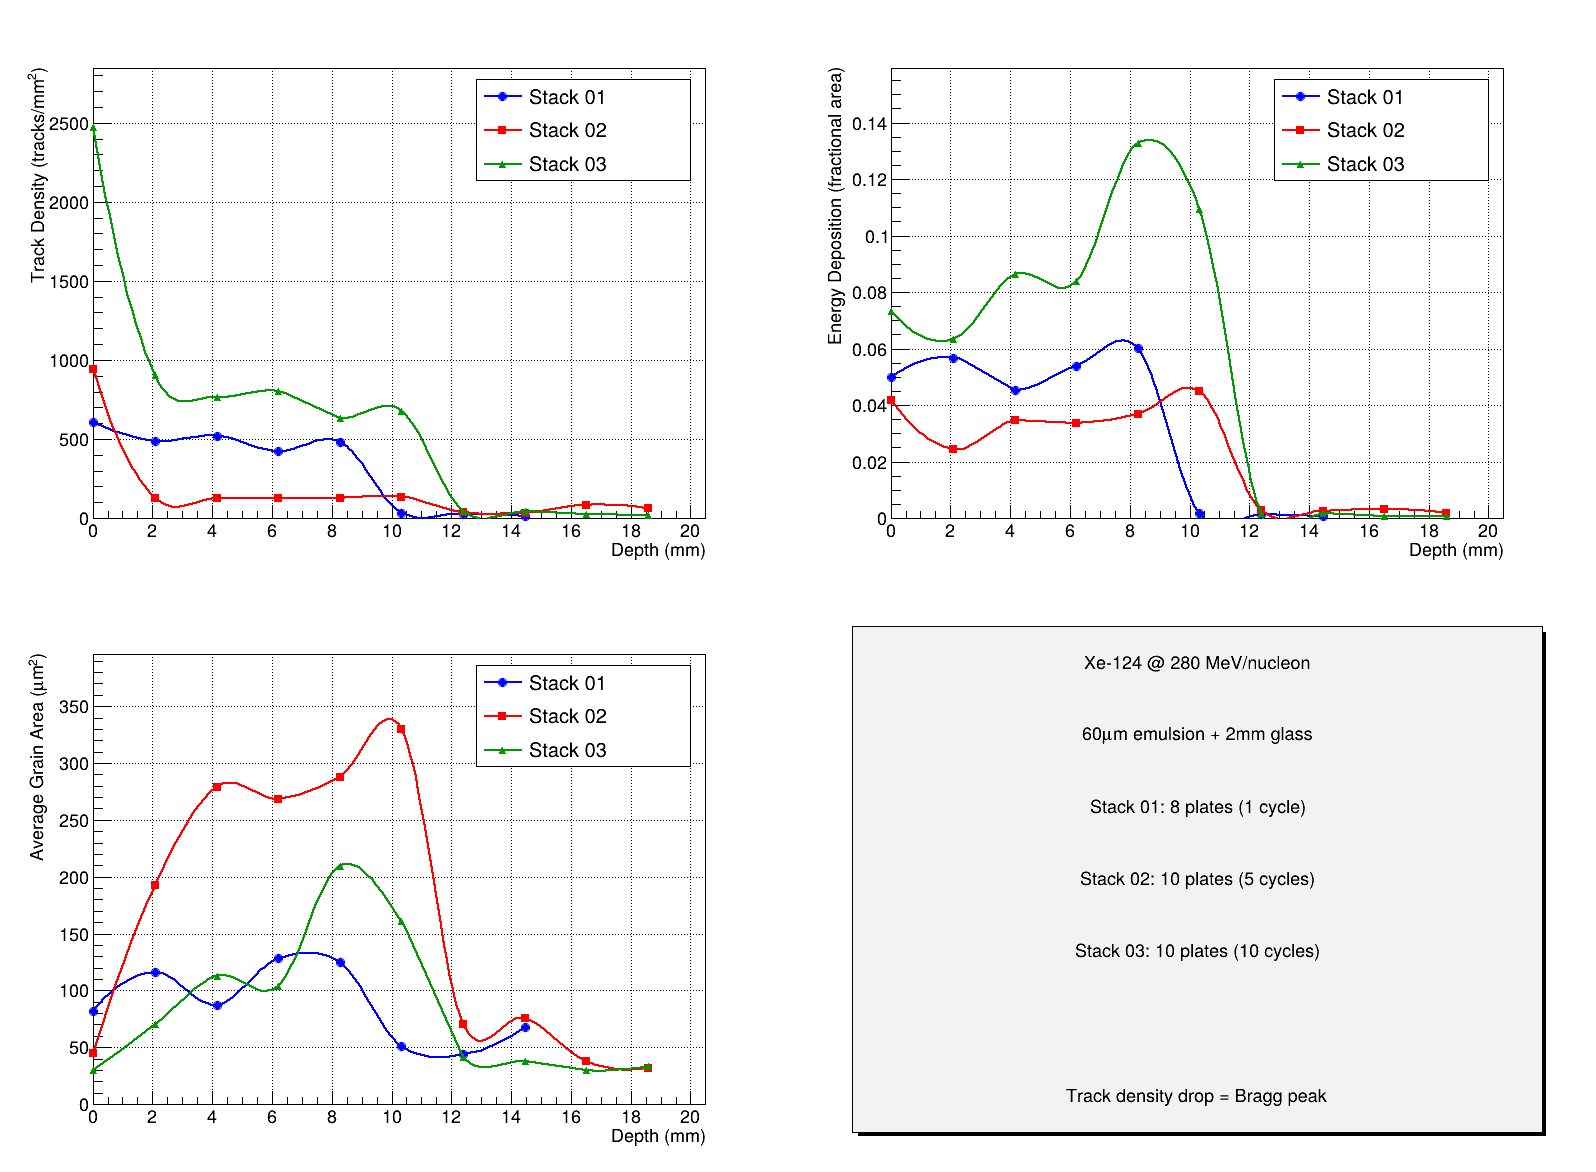
\includegraphics[width=0.85\textwidth]{./bragg_peak_overview.png}
\caption{Four-panel overview of the Bragg peak analysis.
Top-left: track density $\rho$ vs.\ depth;
Top-right: energy deposition fraction $\varepsilon$;
Bottom-left: average grain area $\bar{a}$;
Bottom-right: setup summary with stack configurations.}
\label{fig:overview}
\end{figure}

\begin{table}[H]
\centering
\caption{Bragg peak position summary for all three stacks.}
\label{tab:bragg}
\begin{tabular}{lccccc}
\toprule
Stack & Cycles & $\rho$ before & $\rho$ after & Drop &
Bragg depth \\
 & & (\si{\mm^{-2}}) & (\si{\mm^{-2}}) & factor & (mm) \\
\midrule
Stack\,01 & 1 & 482 & 34 & 14$\times$ & 8--10 \\
Stack\,02 & 5 & 136 & 38 & 3.6$\times$ & 10--12 \\
Stack\,03 & 10 & 680 & 45 & 15$\times$ & 10--12 \\
\bottomrule
\end{tabular}
\end{table}

Stack\,01 peaks approximately 2\,mm earlier than Stacks\,02 and~03.
Possible explanations include a slightly different beam energy, a
different glass thickness in these plates, or the plate orientation
(emulsion layer upstream vs.\ downstream of the glass substrate).

\subsection{Bragg peak ($dE/dx$)}

Figure~\ref{fig:dedx} shows the energy deposition per unit length
($dE/dx$), approximated by the fractional grain area per plate. The
Bragg peak is clearly visible at 8--12\,mm depth, where the energy
loss rate reaches its maximum before the beam stops.

\begin{figure}[H]
\centering
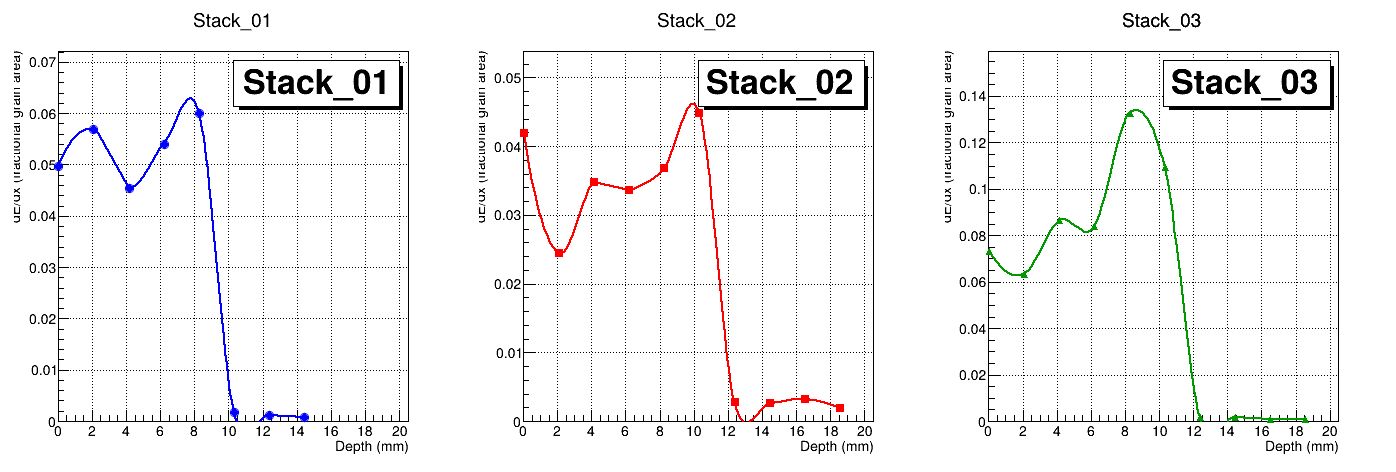
\includegraphics[width=0.85\textwidth]{./bragg_dedx.png}
\caption{$dE/dx$ (fractional grain area) vs depth for each stack.
The Bragg peak appears at 8--10\,mm for Stack\,01 and 10--12\,mm for
Stacks\,02/03. The rapid rise and sharp drop are characteristic of
heavy-ion energy deposition.}
\label{fig:dedx}
\end{figure}

\subsection{Particle classification results}

The GMM-based classification reveals the evolution of particle
populations with depth:

\begin{table}[H]
\centering
\caption{GMM class fractions for Stack\,03 (best statistics).
Full data in \texttt{particle\_classes.csv}. Bold values mark the
plate of maximum abundance for each class.}
\label{tab:gmm}
\begin{tabular}{crrrrrrr}
\toprule
Plate & Depth & \multicolumn{2}{c}{Class\,0} &
\multicolumn{2}{c}{Class\,1} &
\multicolumn{2}{c}{Class\,2} \\
 & (mm) & frac & $\bar{a}$ (\si{\micro\meter\squared}) &
 frac & $\bar{a}$ (\si{\micro\meter\squared}) &
 frac & $\bar{a}$ (\si{\micro\meter\squared}) \\
\midrule
1  & 0.03 & 0.78 & 19.6 & 0.14 & 44.8 & 0.08 & 83.0 \\
2  & 2.09 & 0.02 & 20.3 & \textbf{0.78} & 51.7 & 0.20 & 128.6 \\
3  & 4.15 & 0.06 & 27.3 & 0.68 & 73.0 & 0.26 & 188.6 \\
4  & 6.21 & 0.05 & 27.0 & 0.70 & 70.9 & 0.25 & 180.0 \\
5  & 8.27 & 0.09 & 36.6 & 0.57 & 121.7 & \textbf{0.34} & 326.7 \\
6  & 10.33 & \textbf{0.95} & 114.5 & 0.00 & --- & 0.05 & 474.5 \\
7  & 12.39 & 0.37 & 14.3 & 0.31 & 32.3 & 0.32 & 72.3 \\
8  & 14.45 & 0.36 & 14.1 & 0.32 & 30.4 & 0.32 & 64.3 \\
9  & 16.51 & 0.42 & 12.7 & 0.43 & 26.3 & 0.15 & 43.2 \\
10 & 18.57 & 0.45 & 13.5 & 0.49 & 32.1 & 0.06 & 57.5 \\
\bottomrule
\end{tabular}
\end{table}

\subsection{Physical interpretation}

The results are consistent with the following physical picture:

\begin{itemize}
  \item \textbf{Class\,0 (smallest grains, $\sim$12--50\,\si{\micro\meter\squared}):}
        Light fragments with low $dE/dx$: protons, deuterons,
        tritons, $\alpha$ particles, and light nuclear fragments
        (Z~=~1--5). These dominate after the Bragg peak (plates 7--10)
        where only long-range light fragments survive. The maximum
        abundance (0.95) occurs at plate~6 (10.33\,mm), immediately
        after the Bragg peak where the primary beam has stopped.

  \item \textbf{Class\,1 (medium grains,
        $\sim$40--180\,\si{\micro\meter\squared}):}
        Mid-mass fragments (Z~$\approx$~6--30) produced by abrasion of
        the projectile. This class dominates in the middle of the stack
        (plates 2--5) as the primary beam undergoes nuclear
        fragmentation. The maximum abundance (0.78) occurs at plate~2
        (2.09\,mm), where the fragmentation rate is highest.

  \item \textbf{Class\,2 (largest grains,
        $\sim$180--700+\;\si{\micro\meter\squared}):}
        Primary \textsuperscript{124}Xe and heavy residues
        (Z~$\approx$~30--54). The fraction peaks at the Bragg peak
        region (plate~5, 8.27\,mm, frac~=~0.34) and drops sharply as
        the primary beam stops.
\end{itemize}

The evolution of class fractions with depth follows the
abrasion-ablation model of nuclear fragmentation: the primary Xe
nucleus loses nucleons through peripheral collisions, producing a
distribution of fragments that range from single nucleons to
near-projectile residues.

\subsection{Per-stack observations}

\textbf{Stack\,03} (10 cycles) provides the clearest signal due to its
high statistics. The Bragg peak at 10--12\,mm is unambiguous, with a
15$\times$ drop in track density. The GMM class fractions show a
smooth, physically expected evolution with depth.

\textbf{Stack\,02} (5 cycles) shows a more gradual density drop
(3.6$\times$). The per-cycle density is lower, and the class fraction
trends are noisier. Plate 1 and plate 10 of this stack have
substantially smaller scan areas than the others.

\textbf{Stack\,01} (1 cycle) has the fewest grains per plate. The Bragg
peak appears 2\,mm earlier. Despite the lower statistics, the 14$\times$
density drop is clearly visible.

\subsection{Primary beam (Class\,2) analysis}

Since Class\,2 corresponds to the largest grains (primary
\textsuperscript{124}Xe and heavy fragments with Z~$\approx$~30--54), it
is instructive to examine this population in isolation.

\begin{figure}[H]
\centering
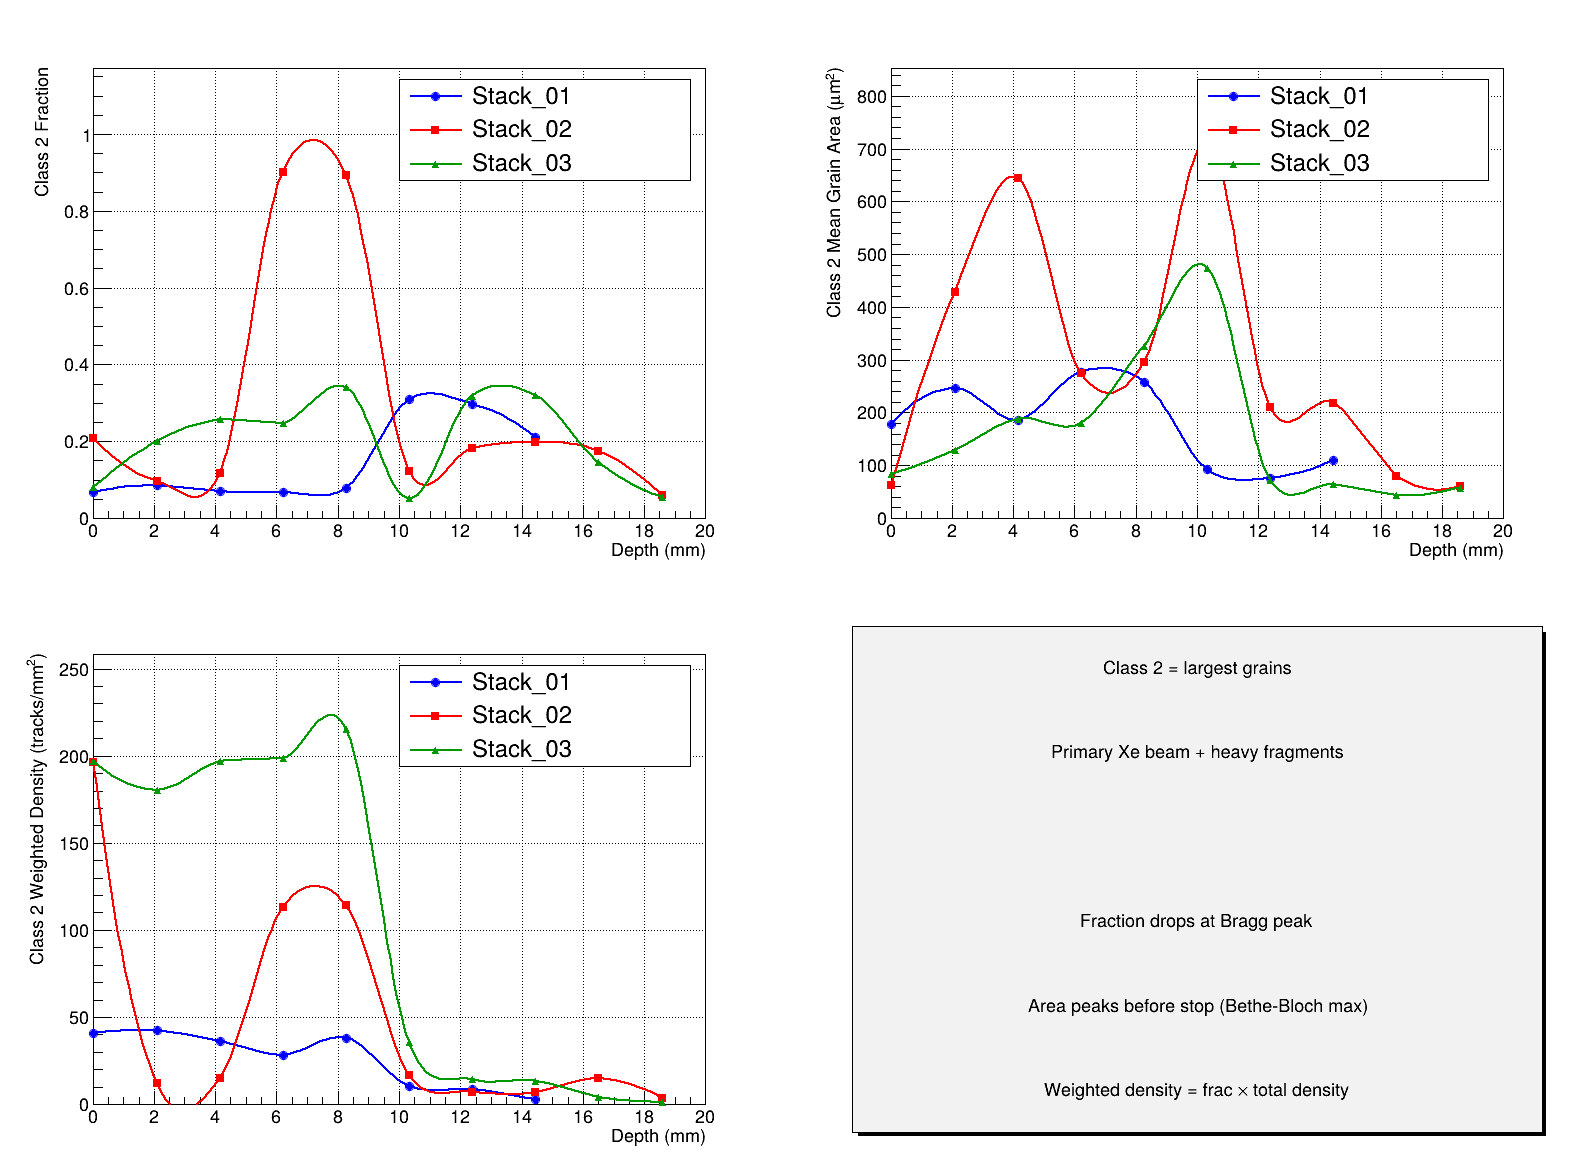
\includegraphics[width=0.95\textwidth]{./class2_analysis.png}
\caption{
  Class\,2 analysis across all stacks.
  \textbf{Top left:} Class\,2 fraction vs depth. The fraction peaks
  at the Bragg peak (plate~5, $\sim$8--10\,mm) and drops sharply
  beyond, confirming that the primary Xe beam stops there.
  \textbf{Top right:} Class\,2 mean grain area vs depth. The area
  increases as the beam slows down (maximum $dE/dx$), then
  decreases as only smaller heavy fragments remain beyond the peak.
  \textbf{Bottom left:} Class\,2 weighted density
  (fraction~$\times$~total track density). This quantity isolates
  the contribution of the primary beam and heavy residues to the
  Bragg curve.
}
\label{fig:class2}
\end{figure}

The key observations are:
\begin{itemize}
  \item \textbf{Class\,2 fraction} (top left) peaks near the Bragg peak
        at 8--10\,mm for Stack\,01 and 10--12\,mm for Stacks\,02/03,
        then drops sharply as the primary Xe stops. Beyond 14\,mm the
        fraction stabilises at 5--15\,\%, representing surviving heavy
        fragments that were produced in peripheral nuclear interactions
        upstream.
  \item \textbf{Mean grain area} (top right) increases with depth as
        the projectile loses energy, reaching a maximum just before the
        Bragg peak (consistent with the Bethe-Bloch maximum). After the
        peak, the mean area decreases as only lighter heavy fragments
        (with lower $dE/dx$) persist.
  \item \textbf{Weighted density} (bottom left) effectively reproduces
        the Bragg curve shape but filtered for the heavy component
        only. The clear peak confirms that the Bragg peak is driven
        by the stopping of the primary beam, not by the accumulation
        of secondary fragments.
\end{itemize}

These results support the interpretation that Class\,2 successfully
isolates the primary Xe beam and its heaviest reaction products, and
that the GMM-based classification provides a physically meaningful
decomposition of the grain-area distribution.

%===================================================================
\section{Conclusions}
\label{sec:conclusions}
%===================================================================

The analysis of three nuclear emulsion stacks exposed to a
\textsuperscript{124}Xe beam at approximately 280--300\,MeV/nucleon at
the JINR Nuclotron leads to the following conclusions:

\begin{enumerate}
  \item \textbf{Bragg peak position.} The primary Xe beam stops between
        10--12\,mm depth in the emulsion--glass stack for Stacks~02
        and~03, consistent with the SRIM-simulated range of
        $\sim$11.5\,mm (Sec.~\ref{sec:srim}). Stack~01 shows a
        slightly earlier stop at 8--10\,mm. The track density drops by
        a factor of 14--15 at the Bragg peak in the two
        high-statistics stacks.

  \item \textbf{Beam intensity.} The per-cycle fluence differs between
        stacks: 605\,\si{\mm^{-2}}/cycle (Stack\,01),
        188\,\si{\mm^{-2}}/cycle (Stack\,02), and
        248\,\si{\mm^{-2}}/cycle (Stack\,03). Stack\,01 received the
        highest instantaneous intensity.

  \item \textbf{Particle classification.} Gaussian Mixture Modelling
        of the $\log_{10}(\text{grain area})$ distribution resolves
        three populations consistent with light fragments (Class~0,
        Z~=~1--5), mid-mass fragments (Class~1, Z~$\approx$~6--30),
        and heavy residues including the primary beam (Class~2,
        Z~$\approx$~30--54). The class fractions evolve with depth in
        accordance with the abrasion-ablation fragmentation model.

  \item \textbf{Beam uniformity.} The lateral beam profile is
        approximately Gaussian and shows no significant hot spots or
        shadowing within the scanned area, confirming adequate
        uniformity.

  \item \textbf{Methodology.} The combination of 4$\times$ objective
        scanning with the Olympus BX63, automatic grain detection in
        ImageJ, and statistical analysis in Python and CERN ROOT
        provides a robust, high-throughput pipeline for heavy-ion
        emulsion analysis. The GMM-based classification offers a
        simple unsupervised approach to fragment identification
        without requiring per-track reconstruction.

  \item \textbf{Data products.} All analysis scripts
        (\texttt{analysis.py}, \texttt{plot\_bragg.C}),
        processed data (\texttt{bragg\_data.csv},
        \texttt{particle\_classes.csv}), and figures are available
        in the \texttt{analysis/} directory. Per-plate diagnostic
        plots (area distributions, radial profiles, beam profiles)
        are available in each stack's \texttt{Plots/} directory.
\end{enumerate}

\newpage
\section*{Acknowledgments}

The author gratefully acknowledges Dr.\ P.\ I.\ Zarubin,
Dr.\ A.\ A.\ Zaitsev, and Dr.\ N.\ Marimuthu for their supervision,
guidance, and support
throughout this work. Special thanks go to the JINR team at the
VBLHEP Experimental Hall for their assistance with the beam
irradiation and to the LHEP nuclear emulsion group for preparing and
processing the emulsion stacks. This work was carried out within the
framework of the BECQUEREL project at the Joint Institute for Nuclear
Research (JINR), Dubna.

\begin{thebibliography}{9}
\bibitem{becquerel}
BECQUEREL project,
``Nuclear Emulsions at LHEP JINR,''
\url{http://becquerel.lhe.jinr.ru/}.

\bibitem{barkas}
W.H.\ Barkas,
\textit{Nuclear Research Emulsions},
Academic Press, New York, 1963.
\url{http://becquerel.lhe.jinr.ru/text/books/Barkas_NUCL_RES_EMULSIONS.pdf}.

\bibitem{srim2008}
J.F.\ Ziegler, J.P.\ Biersack, M.D.\ Ziegler,
\textit{SRIM -- The Stopping and Range of Ions in Matter},
SRIM Co., 2008.
\url{http://www.srim.org}.

\bibitem{imagej}
J.\ Schindelin, I.\ Arganda-Carreras, E.\ Frise et al.,
``Fiji: an open-source platform for biological-image analysis,''
\textit{Nature Methods} \textbf{9}, 676--682 (2012).
\url{https://doi.org/10.1038/nmeth.2019}.

\bibitem{bethe1930}
H.A.\ Bethe,
``Zur Theorie des Durchgangs schneller Korpuskularstrahlen durch
Materie,''
\textit{Ann.\ Phys.} \textbf{397}, 325--400 (1930).
\url{https://doi.org/10.1002/andp.19303970307}.

\bibitem{zarubin2016}
P.I.\ Zarubin,
``Recent applications of nuclear track emulsion technique,''
\textit{Phys.\ At.\ Nucl.} \textbf{79}, 1525--1535 (2016).
\url{https://doi.org/10.1134/S1063778816090179}.

\end{thebibliography}

\end{document}
